\documentclass[aspectratio=1610, twocolumn, handout]{beamer}%, handout
\usepackage{graphics}
\usepackage{pifont}
\usepackage{ulem}
\usepackage{xcolor}
\usepackage{modifycolor}
\usepackage{lipsum}
\usepackage{fontspec}
\usepackage{caption}
\renewcommand{\figurename}{FIGURE}
\captionsetup[figure]{labelfont={color=leftFootlineColor, scriptsize}, textfont={color=normalBlockColor, scriptsize}}
\usepackage{tabularx}
\newcolumntype{Y}{>{\centering\arraybackslash}X}
\usepackage{tikz}
\usepackage{standalone}
\usepackage{svg}
\usepackage{multicol}
\usepackage{catchfilebetweentags}
\usepackage{xifthen}
\usetikzlibrary{arrows}
\usetikzlibrary{backgrounds}
\setmonofont[
  Contextuals={Alternate}
]{FuraCode Nerd Font}
\setsansfont{Roboto Medium}
\usepackage{pgfpages}


\usepackage[cache=false,outputdir=build]{minted}
\definecolor{bg_code}{HTML}{282828}
\usemintedstyle{darcula}
\setminted{
      fontsize=\scriptsize, 
      linenos,
      numbersep=0pt,
      gobble=5,
      framesep=3mm} 
      \renewcommand{\theFancyVerbLine}{\texttt{{{\arabic{FancyVerbLine}}}}}
\usepackage{adjustbox}
\usepackage{environ}%
\usepackage{tikz}
\usetikzlibrary{patterns}
\usepackage[french]{babel}
\usepackage{beamerthemesideblue}


\setbeamerfont{note page}{size=\footnotesize}
\setbeamertemplate{note page}[custom]
\setbeamercolor{note page}{bg=backgroundColor, fg=white}

\newcommand{\insertlicense}{
\includegraphics[height=1cm]{img/by-sa.png}}
\title[]{La rétroingénierie appliquée à Android}
\subtitle{La traque aux traqueurs}
\author{Maxime Catrice}
\date{\today}
\titlegraphic{
\includegraphics[height=0.95cm]{logo.png}\bigbreak\insertlicense}

\setbeamertemplate{title page}[default][colsep=-4bp,rounded=true,shadow=false]
\setbeamercolor{background canvas}{bg=backgroundColor}
\setbeamertemplate{blocks}[rounded][shadow=false]
\beamertemplatenavigationsymbolsempty
\newcounter{acolumn}%  Number of current column
\newlength{\acolumnmaxheight}%   Maximum column height
%%%%%%%%%%%%%%%%%%%%%%%%%


\makeatletter

% `column` replacement to measure height
\newenvironment{@acolumn}[1]{%
    \stepcounter{acolumn}%
    \begin{lrbox}{\@tempboxa}%
    \begin{minipage}{#1}%
}{%
    \end{minipage}
    \end{lrbox}
    \@tempdimc=\dimexpr\ht\@tempboxa+\dp\@tempboxa\relax
    % Save height of this column:
    \expandafter\xdef\csname acolumn@height@\roman{acolumn}\endcsname{\the\@tempdimc}%
    % Save maximum height
    \ifdim\@tempdimc>\acolumnmaxheight
        \global\acolumnmaxheight=\@tempdimc
    \fi
}

% `column` wrapper which sets the height beforehand
\newenvironment{@@acolumn}[1]{%
    \stepcounter{acolumn}%
    % The \autoheight macro contains a \vspace macro with the maximum height minus the natural column height
    \edef\autoheight{\noexpand\vspace*{\dimexpr\acolumnmaxheight-\csname acolumn@height@\roman{acolumn}\endcsname\relax}}%
    % Call original `column`:
    \orig@column{#1}%
}{%
    \endorig@column
}

% Save orignal `column` environment away
\let\orig@column\column
\let\endorig@column\endcolumn

% `columns` variant with automatic height adjustment
\NewEnviron{acolumns}[1][]{%
    % Init vars:
    \setcounter{acolumn}{0}%
    \setlength{\acolumnmaxheight}{0pt}%
    \def\autoheight{\vspace*{0pt}}%
    % Set `column` environment to special measuring environment
    \let\column\@acolumn
    \let\endcolumn\end@acolumn
    \BODY% measure heights
    % Reset counter for second processing round
    \setcounter{acolumn}{0}%
    % Set `column` environment to wrapper
    \let\column\@@acolumn
    \let\endcolumn\end@@acolumn
    % Finally process columns now for real
    \begin{columns}[#1]%
        \BODY
    \end{columns}%
}
\makeatother
%%%%%%%%%%%%%%%%%%%%%%%%%

\NewEnviron{frameNoSB}{
\makeatletter
\setbeamertemplate{sidebar canvas left}{}
\setbeamertemplate{sidebar left}{}
\makeatother
\begin{frame}
    \BODY
%\tableofcontents
\end{frame}
}

\NewEnviron{frameTitle}{
\setbeamertemplate{frametitle}[default][center]
\makeatletter
\setbeamertemplate{headline}{\color{backgroundColor}45\newline 45\newline 45\newline 45\newline 45\newline 45\newline 45\newline 45\newline 45\newline 45}
\setbeamertemplate{sidebar canvas left}{}
\setbeamertemplate{sidebar left}{}



\makeatother
\begin{frame}
\begin{minipage}[c]{\linewidth-\beamerleftmargin+\beamerrightmargin}
\BODY
\end{minipage}
\end{frame}
}

\setbeamerfont{title}{series=\bfseries,parent=structure}
\setbeamerfont{subtitle}{size=\Large,series=,parent=structure}

\makeatletter
\newlength\beamerleftmargin
\setlength\beamerleftmargin{\Gm@lmargin}

\newlength\beamerrightmargin
\setlength\beamerrightmargin{\Gm@rmargin}
\makeatother

\newcommand{\nologo}{\setbeamertemplate{logo}{}}

\newcommand{\slidetitle}[1][]{
  \frametitle{\insertsection\ifthenelse{\equal{#1}{}}{}{: #1}}
}
\newcommand{\mono}[1]{
\texttt{#1}
}

%\setbeameroption{show notes on second screen=left}
\begin{document}
\framegreen
{
  \nologo
  \begin{frameTitle}
  \maketitle
  \end{frameTitle}
}

\begin{frameNoSB} 
\frametitle{\inserttitle}
\begin{columns}
  \begin{column}{.66\linewidth}
    \vspace{0pt}
    \tableofcontents
  \end{column}
  \begin{column}{0.33\linewidth}
  
\includegraphics[width=0.75\linewidth]{img/android.png}
  \end{column}
\end{columns}
\end{frameNoSB}

\framepurple
\documentclass[11pt,aspectratio=1610]{beamer}%, handout
  \usepackage{import}
\usepackage{graphics}
\usepackage{pifont}
\usepackage{ulem}
\usepackage{xcolor}
\usepackage{modifycolor}
\usepackage{lipsum}
\usepackage{fontspec}
\usepackage{caption}
\renewcommand{\figurename}{FIGURE}
\captionsetup[figure]{labelfont={color=leftFootlineColor, scriptsize}, textfont={color=normalBlockColor, scriptsize}}
\usepackage{tabularx}
\newcolumntype{Y}{>{\centering\arraybackslash}X}
\usepackage{tikz}
\usepackage{standalone}
\usepackage{svg}
\usepackage{multicol}
\usepackage{catchfilebetweentags}
\usepackage{xifthen}
\usetikzlibrary{arrows}
\usetikzlibrary{backgrounds}
\setmonofont[
  Contextuals={Alternate}
]{FuraCode Nerd Font}
\setsansfont{Roboto Medium}
\usepackage{pgfpages}


\usepackage[cache=false,outputdir=build]{minted}
\definecolor{bg_code}{HTML}{282828}
\usemintedstyle{darcula}
\setminted{
      fontsize=\scriptsize, 
      linenos,
      numbersep=0pt,
      gobble=5,
      framesep=3mm} 
      \renewcommand{\theFancyVerbLine}{\texttt{{{\arabic{FancyVerbLine}}}}}
\usepackage{adjustbox}
\usepackage{environ}%
\usepackage{tikz}
\usetikzlibrary{patterns}
\usepackage[french]{babel}
\usepackage{beamerthemesideblue}


\setbeamerfont{note page}{size=\footnotesize}
\setbeamertemplate{note page}[custom]
\setbeamercolor{note page}{bg=backgroundColor, fg=white}

\newcommand{\insertlicense}{
\includegraphics[height=1cm]{img/by-sa.png}}
\title[]{La rétroingénierie appliquée à Android}
\subtitle{La traque aux traqueurs}
\author{Maxime Catrice}
\date{\today}
\titlegraphic{
\includegraphics[height=0.95cm]{logo.png}\bigbreak\insertlicense}

\setbeamertemplate{title page}[default][colsep=-4bp,rounded=true,shadow=false]
\setbeamercolor{background canvas}{bg=backgroundColor}
\setbeamertemplate{blocks}[rounded][shadow=false]
\beamertemplatenavigationsymbolsempty
\newcounter{acolumn}%  Number of current column
\newlength{\acolumnmaxheight}%   Maximum column height
%%%%%%%%%%%%%%%%%%%%%%%%%


\makeatletter

% `column` replacement to measure height
\newenvironment{@acolumn}[1]{%
    \stepcounter{acolumn}%
    \begin{lrbox}{\@tempboxa}%
    \begin{minipage}{#1}%
}{%
    \end{minipage}
    \end{lrbox}
    \@tempdimc=\dimexpr\ht\@tempboxa+\dp\@tempboxa\relax
    % Save height of this column:
    \expandafter\xdef\csname acolumn@height@\roman{acolumn}\endcsname{\the\@tempdimc}%
    % Save maximum height
    \ifdim\@tempdimc>\acolumnmaxheight
        \global\acolumnmaxheight=\@tempdimc
    \fi
}

% `column` wrapper which sets the height beforehand
\newenvironment{@@acolumn}[1]{%
    \stepcounter{acolumn}%
    % The \autoheight macro contains a \vspace macro with the maximum height minus the natural column height
    \edef\autoheight{\noexpand\vspace*{\dimexpr\acolumnmaxheight-\csname acolumn@height@\roman{acolumn}\endcsname\relax}}%
    % Call original `column`:
    \orig@column{#1}%
}{%
    \endorig@column
}

% Save orignal `column` environment away
\let\orig@column\column
\let\endorig@column\endcolumn

% `columns` variant with automatic height adjustment
\NewEnviron{acolumns}[1][]{%
    % Init vars:
    \setcounter{acolumn}{0}%
    \setlength{\acolumnmaxheight}{0pt}%
    \def\autoheight{\vspace*{0pt}}%
    % Set `column` environment to special measuring environment
    \let\column\@acolumn
    \let\endcolumn\end@acolumn
    \BODY% measure heights
    % Reset counter for second processing round
    \setcounter{acolumn}{0}%
    % Set `column` environment to wrapper
    \let\column\@@acolumn
    \let\endcolumn\end@@acolumn
    % Finally process columns now for real
    \begin{columns}[#1]%
        \BODY
    \end{columns}%
}
\makeatother
%%%%%%%%%%%%%%%%%%%%%%%%%

\NewEnviron{frameNoSB}{
\makeatletter
\setbeamertemplate{sidebar canvas left}{}
\setbeamertemplate{sidebar left}{}
\makeatother
\begin{frame}
    \BODY
%\tableofcontents
\end{frame}
}

\NewEnviron{frameTitle}{
\setbeamertemplate{frametitle}[default][center]
\makeatletter
\setbeamertemplate{headline}{\color{backgroundColor}45\newline 45\newline 45\newline 45\newline 45\newline 45\newline 45\newline 45\newline 45\newline 45}
\setbeamertemplate{sidebar canvas left}{}
\setbeamertemplate{sidebar left}{}



\makeatother
\begin{frame}
\begin{minipage}[c]{\linewidth-\beamerleftmargin+\beamerrightmargin}
\BODY
\end{minipage}
\end{frame}
}

\setbeamerfont{title}{series=\bfseries,parent=structure}
\setbeamerfont{subtitle}{size=\Large,series=,parent=structure}

\makeatletter
\newlength\beamerleftmargin
\setlength\beamerleftmargin{\Gm@lmargin}

\newlength\beamerrightmargin
\setlength\beamerrightmargin{\Gm@rmargin}
\makeatother

\newcommand{\nologo}{\setbeamertemplate{logo}{}}

\newcommand{\slidetitle}[1][]{
  \frametitle{\insertsection\ifthenelse{\equal{#1}{}}{}{: #1}}
}
\newcommand{\mono}[1]{
\texttt{#1}
}

\setbeameroption{show notes on second screen=top}
\begin{document}
\section{Qu'est ce que la rétroingénierie ?}
  \begin{frame}[t]
      \slidetitle[]
      \note{\onslide<1->{\ExecuteMetaData[001-retro_notes.tex]{Definition}}}
      \note{\onslide<5->{\ExecuteMetaData[001-retro_notes.tex]{Objectifs}}}
      \begin{block}{Principe :}<2->
        \onslide<3->{
        Analyser un programme sans ses sources, pour en comprendre le fonctionnement interne.
        }
      \end{block}
      \vfill
      \begin{columns}
        \begin{column}{.7\linewidth}
          \begin{block}{Objectifs :}<4->
            \begin{itemize}
            \item<5-> Interopérabilité
            \item<6-> Documentation
            \item<7-> Veille compétitive
            \item<8-> Recherche de failles de sécurités
            \item<9-> Piratage
            \end{itemize}
          \end{block}
        \end{column}
        \begin{column}{.25\linewidth}
          \centering
          
\includegraphics[width=\linewidth]{img/android_loupe.png}
        \end{column}
      \end{columns}
      \vfill
  \end{frame}
  % \begin{frame}
  %   \slidetitle[]
  %   Test
  % \end{frame}
\end{document}

\framebrown
\documentclass[aspectratio=1610]{beamer}%, handout
  \usepackage{graphics}
\usepackage{pifont}
\usepackage{ulem}
\usepackage{xcolor}
\usepackage{modifycolor}
\usepackage{lipsum}
\usepackage{fontspec}
\usepackage{caption}
\renewcommand{\figurename}{FIGURE}
\captionsetup[figure]{labelfont={color=leftFootlineColor, scriptsize}, textfont={color=normalBlockColor, scriptsize}}
\usepackage{tabularx}
\newcolumntype{Y}{>{\centering\arraybackslash}X}
\usepackage{tikz}
\usepackage{standalone}
\usepackage{svg}
\usepackage{multicol}
\usepackage{catchfilebetweentags}
\usepackage{xifthen}
\usetikzlibrary{arrows}
\usetikzlibrary{backgrounds}
\setmonofont[
  Contextuals={Alternate}
]{FuraCode Nerd Font}
\setsansfont{Roboto Medium}
\usepackage{pgfpages}


\usepackage[cache=false,outputdir=build]{minted}
\definecolor{bg_code}{HTML}{282828}
\usemintedstyle{darcula}
\setminted{
      fontsize=\scriptsize, 
      linenos,
      numbersep=0pt,
      gobble=5,
      framesep=3mm} 
      \renewcommand{\theFancyVerbLine}{\texttt{{{\arabic{FancyVerbLine}}}}}
\usepackage{adjustbox}
\usepackage{environ}%
\usepackage{tikz}
\usetikzlibrary{patterns}
\usepackage[french]{babel}
\usepackage{beamerthemesideblue}


\setbeamerfont{note page}{size=\footnotesize}
\setbeamertemplate{note page}[custom]
\setbeamercolor{note page}{bg=backgroundColor, fg=white}

\newcommand{\insertlicense}{
\includegraphics[height=1cm]{img/by-sa.png}}
\title[]{La rétroingénierie appliquée à Android}
\subtitle{La traque aux traqueurs}
\author{Maxime Catrice}
\date{\today}
\titlegraphic{
\includegraphics[height=0.95cm]{logo.png}\bigbreak\insertlicense}

\setbeamertemplate{title page}[default][colsep=-4bp,rounded=true,shadow=false]
\setbeamercolor{background canvas}{bg=backgroundColor}
\setbeamertemplate{blocks}[rounded][shadow=false]
\beamertemplatenavigationsymbolsempty
\newcounter{acolumn}%  Number of current column
\newlength{\acolumnmaxheight}%   Maximum column height
%%%%%%%%%%%%%%%%%%%%%%%%%


\makeatletter

% `column` replacement to measure height
\newenvironment{@acolumn}[1]{%
    \stepcounter{acolumn}%
    \begin{lrbox}{\@tempboxa}%
    \begin{minipage}{#1}%
}{%
    \end{minipage}
    \end{lrbox}
    \@tempdimc=\dimexpr\ht\@tempboxa+\dp\@tempboxa\relax
    % Save height of this column:
    \expandafter\xdef\csname acolumn@height@\roman{acolumn}\endcsname{\the\@tempdimc}%
    % Save maximum height
    \ifdim\@tempdimc>\acolumnmaxheight
        \global\acolumnmaxheight=\@tempdimc
    \fi
}

% `column` wrapper which sets the height beforehand
\newenvironment{@@acolumn}[1]{%
    \stepcounter{acolumn}%
    % The \autoheight macro contains a \vspace macro with the maximum height minus the natural column height
    \edef\autoheight{\noexpand\vspace*{\dimexpr\acolumnmaxheight-\csname acolumn@height@\roman{acolumn}\endcsname\relax}}%
    % Call original `column`:
    \orig@column{#1}%
}{%
    \endorig@column
}

% Save orignal `column` environment away
\let\orig@column\column
\let\endorig@column\endcolumn

% `columns` variant with automatic height adjustment
\NewEnviron{acolumns}[1][]{%
    % Init vars:
    \setcounter{acolumn}{0}%
    \setlength{\acolumnmaxheight}{0pt}%
    \def\autoheight{\vspace*{0pt}}%
    % Set `column` environment to special measuring environment
    \let\column\@acolumn
    \let\endcolumn\end@acolumn
    \BODY% measure heights
    % Reset counter for second processing round
    \setcounter{acolumn}{0}%
    % Set `column` environment to wrapper
    \let\column\@@acolumn
    \let\endcolumn\end@@acolumn
    % Finally process columns now for real
    \begin{columns}[#1]%
        \BODY
    \end{columns}%
}
\makeatother
%%%%%%%%%%%%%%%%%%%%%%%%%

\NewEnviron{frameNoSB}{
\makeatletter
\setbeamertemplate{sidebar canvas left}{}
\setbeamertemplate{sidebar left}{}
\makeatother
\begin{frame}
    \BODY
%\tableofcontents
\end{frame}
}

\NewEnviron{frameTitle}{
\setbeamertemplate{frametitle}[default][center]
\makeatletter
\setbeamertemplate{headline}{\color{backgroundColor}45\newline 45\newline 45\newline 45\newline 45\newline 45\newline 45\newline 45\newline 45\newline 45}
\setbeamertemplate{sidebar canvas left}{}
\setbeamertemplate{sidebar left}{}



\makeatother
\begin{frame}
\begin{minipage}[c]{\linewidth-\beamerleftmargin+\beamerrightmargin}
\BODY
\end{minipage}
\end{frame}
}

\setbeamerfont{title}{series=\bfseries,parent=structure}
\setbeamerfont{subtitle}{size=\Large,series=,parent=structure}

\makeatletter
\newlength\beamerleftmargin
\setlength\beamerleftmargin{\Gm@lmargin}

\newlength\beamerrightmargin
\setlength\beamerrightmargin{\Gm@rmargin}
\makeatother

\newcommand{\nologo}{\setbeamertemplate{logo}{}}

\newcommand{\slidetitle}[1][]{
  \frametitle{\insertsection\ifthenelse{\equal{#1}{}}{}{: #1}}
}
\newcommand{\mono}[1]{
\texttt{#1}
}

  \setbeameroption{show notes on second screen=top}
  \begin{document}

  \section{Légalité et rétroingénierie}
  \begin{frame}[t]
    \slidetitle[]%{Légalité et rétroingénierie}
    \note{\ExecuteMetaData[002-legal_notes.tex]{propIntelect}}
    \note{\onslide<5->{\ExecuteMetaData[002-legal_notes.tex]{loi}}}
    \note{\onslide<10->{\ExecuteMetaData[002-legal_notes.tex]{Resume}}}
%    \note{\onslide+<4->{\ExecuteMetaData[002-legal_notes.tex]{interropérabilité}}}
    \begin{columns}
      \begin{column}{0.7\linewidth}
        \begin{block}{Logiciels et propriété intellectuelle}<2->
          \begin{itemize}
          \item<3-> Logiciel protégeable
          \item<4-> Fonctionnalité en tant que telle non protégeable
          \end{itemize}
        \end{block}
        \begin{block}{Article 122-6-1 du code de la propriété intellectuelle}<5->
          \begin{itemize}
          \item<6-> Acquisition légale du logiciel
          \item<7-> Soit:
          \begin{itemize}
          \item<8-> La license ne l'interdit pas
          \item<9-> Réalisation à des fins d'interropérabilité
          \end{itemize} 
          \end{itemize}
        \end{block}
      \end{column}
      \begin{column}{0.25\linewidth}
        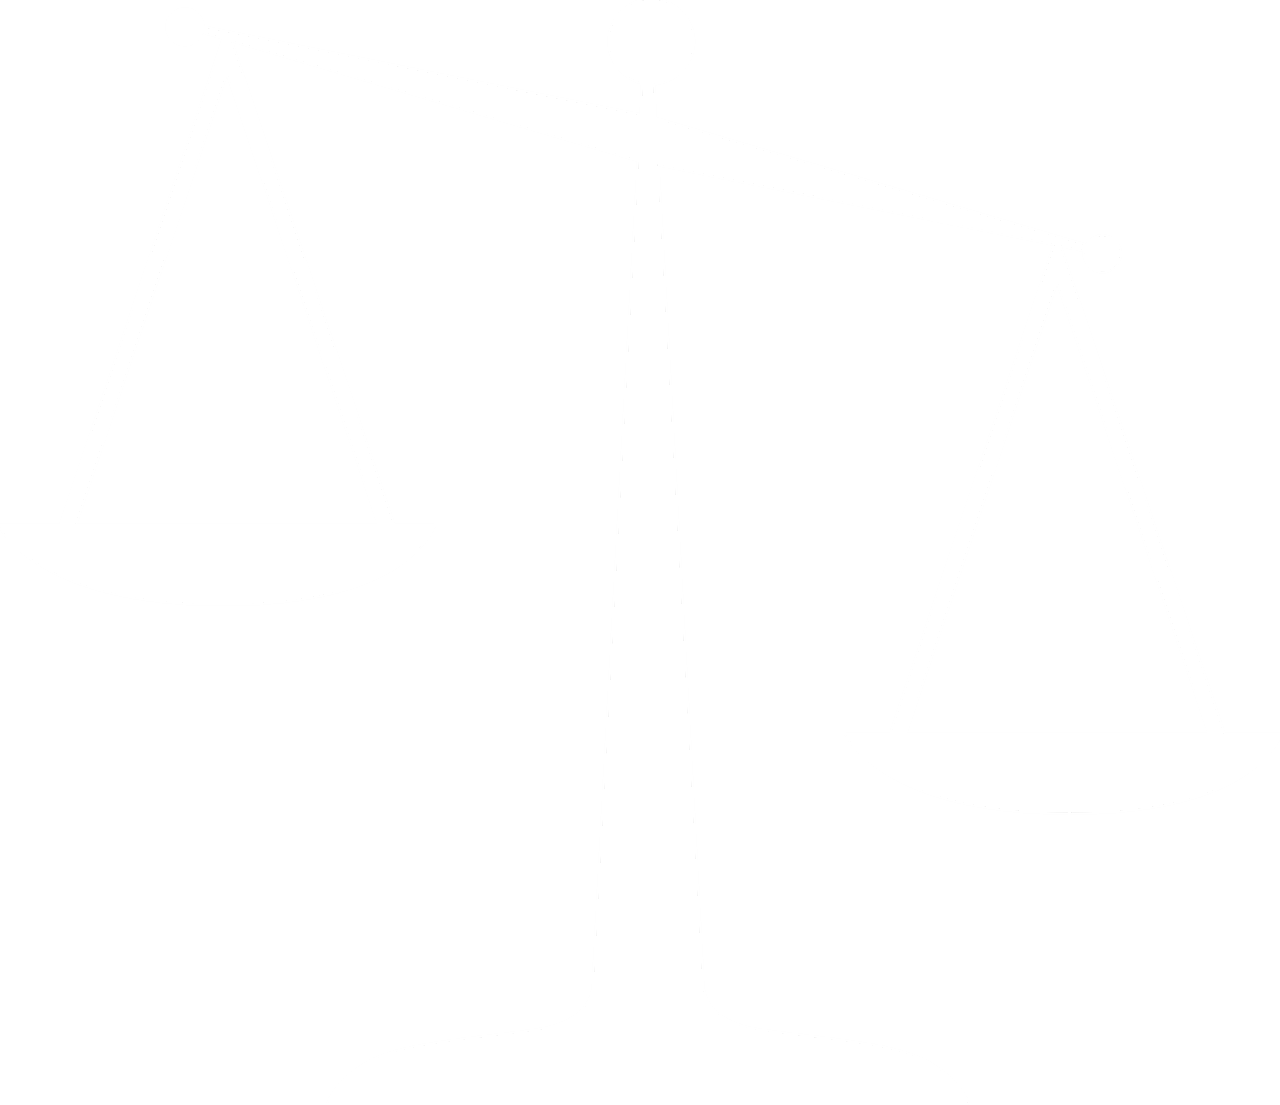
\includegraphics[width=0.95\linewidth]{img/justice.png}
      \end{column}
    \end{columns}
      \onslide+<10->{\begin{center}
        « On n'a donc pas le droit en France de démontrer techniquement qu'un logiciel présente des failles
  de sécurité, ou que la publicité pour ces logiciels est mensongère. Dormez tranquilles, citoyens, tous
  vos logiciels sont parfaits. » 
      \end{center}
      \vspace{-1.5\baselineskip}
      \hspace{0.66\linewidth}Guillermito
      }
    \end{frame}
  \end{document}

    \begin{frame}
    \slidetitle[Les Bug BugBounty]
    \note{\ExecuteMetaData[002-legal_notes.tex]{BugBounty}}
    \note{\onslide<4->{\ExecuteMetaData[002-legal_notes.tex]{Tweet}}}
    \pause
    \begin{block}{Qu'est ce qu'un Bug Bounty?}
      \centering
      \onslide<3->{Un bug bounty est un programme proposé par de nombreux sites web et développeurs de logiciel
       qui permet à des personnes de recevoir reconnaissance et compensation après avoir reporté
        des bugs, surtout ceux concernant des exploits et des vulnérabilités}
    \end{block}
    \vfill
    \centering
    \onslide<4->{
      \begin{figure}
        
\includegraphics[width=0.5\linewidth]{tweet.png}
        \caption{Tweet montrant une faille dans macOS}
      \end{figure}}
      \end{frame}
  \end{document}


\framebluegray
\documentclass[aspectratio=1610]{beamer}%, handout
  \usepackage{graphics}
\usepackage{pifont}
\usepackage{ulem}
\usepackage{xcolor}
\usepackage{modifycolor}
\usepackage{lipsum}
\usepackage{fontspec}
\usepackage{caption}
\renewcommand{\figurename}{FIGURE}
\captionsetup[figure]{labelfont={color=leftFootlineColor, scriptsize}, textfont={color=normalBlockColor, scriptsize}}
\usepackage{tabularx}
\newcolumntype{Y}{>{\centering\arraybackslash}X}
\usepackage{tikz}
\usepackage{standalone}
\usepackage{svg}
\usepackage{multicol}
\usepackage{catchfilebetweentags}
\usepackage{xifthen}
\usetikzlibrary{arrows}
\usetikzlibrary{backgrounds}
\setmonofont[
  Contextuals={Alternate}
]{FuraCode Nerd Font}
\setsansfont{Roboto Medium}
\usepackage{pgfpages}


\usepackage[cache=false,outputdir=build]{minted}
\definecolor{bg_code}{HTML}{282828}
\usemintedstyle{darcula}
\setminted{
      fontsize=\scriptsize, 
      linenos,
      numbersep=0pt,
      gobble=5,
      framesep=3mm} 
      \renewcommand{\theFancyVerbLine}{\texttt{{{\arabic{FancyVerbLine}}}}}
\usepackage{adjustbox}
\usepackage{environ}%
\usepackage{tikz}
\usetikzlibrary{patterns}
\usepackage[french]{babel}
\usepackage{beamerthemesideblue}


\setbeamerfont{note page}{size=\footnotesize}
\setbeamertemplate{note page}[custom]
\setbeamercolor{note page}{bg=backgroundColor, fg=white}

\newcommand{\insertlicense}{
\includegraphics[height=1cm]{img/by-sa.png}}
\title[]{La rétroingénierie appliquée à Android}
\subtitle{La traque aux traqueurs}
\author{Maxime Catrice}
\date{\today}
\titlegraphic{
\includegraphics[height=0.95cm]{logo.png}\bigbreak\insertlicense}

\setbeamertemplate{title page}[default][colsep=-4bp,rounded=true,shadow=false]
\setbeamercolor{background canvas}{bg=backgroundColor}
\setbeamertemplate{blocks}[rounded][shadow=false]
\beamertemplatenavigationsymbolsempty
\newcounter{acolumn}%  Number of current column
\newlength{\acolumnmaxheight}%   Maximum column height
%%%%%%%%%%%%%%%%%%%%%%%%%


\makeatletter

% `column` replacement to measure height
\newenvironment{@acolumn}[1]{%
    \stepcounter{acolumn}%
    \begin{lrbox}{\@tempboxa}%
    \begin{minipage}{#1}%
}{%
    \end{minipage}
    \end{lrbox}
    \@tempdimc=\dimexpr\ht\@tempboxa+\dp\@tempboxa\relax
    % Save height of this column:
    \expandafter\xdef\csname acolumn@height@\roman{acolumn}\endcsname{\the\@tempdimc}%
    % Save maximum height
    \ifdim\@tempdimc>\acolumnmaxheight
        \global\acolumnmaxheight=\@tempdimc
    \fi
}

% `column` wrapper which sets the height beforehand
\newenvironment{@@acolumn}[1]{%
    \stepcounter{acolumn}%
    % The \autoheight macro contains a \vspace macro with the maximum height minus the natural column height
    \edef\autoheight{\noexpand\vspace*{\dimexpr\acolumnmaxheight-\csname acolumn@height@\roman{acolumn}\endcsname\relax}}%
    % Call original `column`:
    \orig@column{#1}%
}{%
    \endorig@column
}

% Save orignal `column` environment away
\let\orig@column\column
\let\endorig@column\endcolumn

% `columns` variant with automatic height adjustment
\NewEnviron{acolumns}[1][]{%
    % Init vars:
    \setcounter{acolumn}{0}%
    \setlength{\acolumnmaxheight}{0pt}%
    \def\autoheight{\vspace*{0pt}}%
    % Set `column` environment to special measuring environment
    \let\column\@acolumn
    \let\endcolumn\end@acolumn
    \BODY% measure heights
    % Reset counter for second processing round
    \setcounter{acolumn}{0}%
    % Set `column` environment to wrapper
    \let\column\@@acolumn
    \let\endcolumn\end@@acolumn
    % Finally process columns now for real
    \begin{columns}[#1]%
        \BODY
    \end{columns}%
}
\makeatother
%%%%%%%%%%%%%%%%%%%%%%%%%

\NewEnviron{frameNoSB}{
\makeatletter
\setbeamertemplate{sidebar canvas left}{}
\setbeamertemplate{sidebar left}{}
\makeatother
\begin{frame}
    \BODY
%\tableofcontents
\end{frame}
}

\NewEnviron{frameTitle}{
\setbeamertemplate{frametitle}[default][center]
\makeatletter
\setbeamertemplate{headline}{\color{backgroundColor}45\newline 45\newline 45\newline 45\newline 45\newline 45\newline 45\newline 45\newline 45\newline 45}
\setbeamertemplate{sidebar canvas left}{}
\setbeamertemplate{sidebar left}{}



\makeatother
\begin{frame}
\begin{minipage}[c]{\linewidth-\beamerleftmargin+\beamerrightmargin}
\BODY
\end{minipage}
\end{frame}
}

\setbeamerfont{title}{series=\bfseries,parent=structure}
\setbeamerfont{subtitle}{size=\Large,series=,parent=structure}

\makeatletter
\newlength\beamerleftmargin
\setlength\beamerleftmargin{\Gm@lmargin}

\newlength\beamerrightmargin
\setlength\beamerrightmargin{\Gm@rmargin}
\makeatother

\newcommand{\nologo}{\setbeamertemplate{logo}{}}

\newcommand{\slidetitle}[1][]{
  \frametitle{\insertsection\ifthenelse{\equal{#1}{}}{}{: #1}}
}
\newcommand{\mono}[1]{
\texttt{#1}
}

  \setbeameroption{show notes on second screen=top}
  \begin{document}
  
  \section{Les aplications Android}
  \begin{frame}
    \slidetitle[Composition]
    \note{\ExecuteMetaData[003-apk_notes.tex]{Composition}}
    \pause
    \begin{columns}
      \begin{column}{0.4\linewidth}
        \texttt{\scriptsize
        \begin{itemize}
        \item [~]
\includegraphics[height=0.8 \baselineskip]{img/xml@2x.pdf}~AndroidManifest.xml
        \item 
\includegraphics[height=0.8 \baselineskip]{img/sourceFolder@2x.png}~assets
        \item [~]
\includegraphics[height=0.8 \baselineskip]{img/javaClass@2x.pdf}~classes.dex
        \item 
\includegraphics[height=0.8 \baselineskip]{img/sourceFolder@2x.png}~lib/
        \item 
\includegraphics[height=0.8 \baselineskip]{img/sourceFolder@2x.png}~META-INF/
        \item 
\includegraphics[height=0.8 \baselineskip]{img/ResourcesRoot.pdf}~res/
        \item [~] 
\includegraphics[height=0.8\baselineskip]{img/component@2x.png}~resources.arsc
        \end{itemize}
        }
      \end{column}
      \begin{column}{0.6\linewidth}
        {\scriptsize
        \begin{itemize}%[label=--]
        \item<3-> [~] Permissions, Activités...
        \item<4-> [~] Ressources non compilées, non standards
        \item<5-> [~] Code binaire de l'application
        \item<6-> [~] Librairies externes
        \item<7-> [~] Informations autour de l'application
        \item<8-> [~] Ressources standards, non compilées
        \item<9-> [~] Ressources compilées
        \end{itemize}
        }
      \end{column}
    \end{columns}
  \end{frame}
  \begin{frame}
    \slidetitle[Compilation]
    \note{\ExecuteMetaData[003-apk_notes.tex]{Compilation}}
    \pause
    \note{\onslide+<3->{\ExecuteMetaData[003-apk_notes.tex]{ARTVSDalvik}}}
    \begin{columns}
      \begin{column}{0.5\linewidth}
        \begin{figure}
          \vspace{-0.5cm}
          \begin{tikzpicture}[scale=0.6, every node/.style={scale=0.6}, show background rectangle,background rectangle/.style={fill=backgroundColor},color=white,]
    \tikzstyle{myarrows}=[thick, line width=1.7mm,-open triangle 90,
    postaction={draw, line width=6.5mm, shorten >=4mm, -},
    postaction={draw, backgroundColor, shorten >= 1.3mm, -triangle 90, line width=1mm},
    postaction={draw, line width=5mm, backgroundColor, shorten >= 4mm, -}]
    
\draw [ultra thick, rounded corners=5] (0,0) rectangle node{
\begin{tabular}{c}
Code source\\Java (.java)
\end{tabular}
} (3,-1.5);
\node[inner sep=0,minimum size=0] at (1.5,-1.5) (CS) {}; % invisible node
\draw [ultra thick, rounded corners=5] (0,-3.5) rectangle node{
\begin{tabular}{c}
Bytecode\\Java (.class)
\end{tabular}
} (3,-5);
\node[inner sep=0,minimum size=0] at (1.5,-3.5) (BJ0) {}; % invisible node

\draw[myarrows] (CS) to (BJ0);
\node[inner sep=0,minimum size=0] at (1.5,-5) (BJ1) {}; % invisible node

\node[inner sep=0,minimum size=0] at (1.5,-10) (JB) {}; % invisible node
\draw[myarrows] (BJ1) to (JB);


\draw [ultra thick] (0,-10) rectangle node{
Java Bytecode
} (3,-11);
\draw [ultra thick] (0,-11) rectangle node{
Java VM
} (3,-12);

\draw [ultra thick, rounded corners=5] (6,0) rectangle node{
\begin{tabular}{c}
Code source\\Java (.java)
\end{tabular}
} (9,-1.5);
\node[inner sep=0,minimum size=0] at (7.5,-1.5) (CCSS) {}; % invisible node

\node[inner sep=0,minimum size=0] at (7.5,-3.5) (BJ0) {}; % invisible node

\draw[myarrows] (CCSS) to (BJ0);

\draw [ultra thick, rounded corners=5] (6,-3.5) rectangle node{
\begin{tabular}{c}
Bytecode\\Java (.class)
\end{tabular}
} (9,-5);

\node[inner sep=0,minimum size=0] at (7.5,-5) (BJ1) {}; % invisible node


\node[inner sep=0,minimum size=0] at (7.5,-7) (BD0) {}; % invisible node
\draw[myarrows] (BJ1) to (BD0);
\draw [ultra thick, rounded corners=5] (6,-7) rectangle node{
\begin{tabular}{c}
Bytecode\\Dalvik (.dex)
\end{tabular}
} (9,-8.5);
\node[inner sep=0,minimum size=0] at (7.5,-8.5) (BD1) {}; % invisible node

\node[inner sep=0,minimum size=0] at (7.5,-10) (DE) {}; % invisible node
\draw[myarrows] (BD1) to (DE);
\draw [ultra thick] (6,-10) rectangle node{
Dalvik Exe
} (9,-11);
\draw [ultra thick] (6,-11) rectangle node{
Dalvik/ART VM
} (9,-12);

\node[font=\Large] at (5.75,-2.5) {javac};
\node[font=\Large] at (3.25,-2.5) {javac};
\node[font=\Large] at (6,-6) {dx};
\end{tikzpicture}
          \vspace{-0.25cm}
          \caption{Compilation Java \& Android}
        \end{figure}
      \end{column}
    \begin{column}{0.5\linewidth}
      \pause
      \begin{block}{
        ~~~~~~~~~~~~~ART \hfill ~vs \hfill Dalvik~~~~~~~~~~~~
      }
        \pause
        \begin{tabularx}{\textwidth}{YY}
        JIT & AOT \\
        \texttt{<=}4.4 & \texttt{>=}4.4
        \end{tabularx}
        \centering
        \pause
        \texttt{>=}7.0: AOT \& JIT
      \end{block}
    \end{column}
  \end{columns}
\end{frame}
\end{document}

\frameyellow
\documentclass[aspectratio=1610,]{beamer}%, handout
\usepackage{graphics}
\usepackage{pifont}
\usepackage{ulem}
\usepackage{xcolor}
\usepackage{modifycolor}
\usepackage{lipsum}
\usepackage{fontspec}
\usepackage{caption}
\renewcommand{\figurename}{FIGURE}
\captionsetup[figure]{labelfont={color=leftFootlineColor, scriptsize}, textfont={color=normalBlockColor, scriptsize}}
\usepackage{tabularx}
\newcolumntype{Y}{>{\centering\arraybackslash}X}
\usepackage{tikz}
\usepackage{standalone}
\usepackage{svg}
\usepackage{multicol}
\usepackage{catchfilebetweentags}
\usepackage{xifthen}
\usetikzlibrary{arrows}
\usetikzlibrary{backgrounds}
\setmonofont[
  Contextuals={Alternate}
]{FuraCode Nerd Font}
\setsansfont{Roboto Medium}
\usepackage{pgfpages}


\usepackage[cache=false,outputdir=build]{minted}
\definecolor{bg_code}{HTML}{282828}
\usemintedstyle{darcula}
\setminted{
      fontsize=\scriptsize, 
      linenos,
      numbersep=0pt,
      gobble=5,
      framesep=3mm} 
      \renewcommand{\theFancyVerbLine}{\texttt{{{\arabic{FancyVerbLine}}}}}
\usepackage{adjustbox}
\usepackage{environ}%
\usepackage{tikz}
\usetikzlibrary{patterns}
\usepackage[french]{babel}
\usepackage{beamerthemesideblue}


\setbeamerfont{note page}{size=\footnotesize}
\setbeamertemplate{note page}[custom]
\setbeamercolor{note page}{bg=backgroundColor, fg=white}

\newcommand{\insertlicense}{
\includegraphics[height=1cm]{img/by-sa.png}}
\title[]{La rétroingénierie appliquée à Android}
\subtitle{La traque aux traqueurs}
\author{Maxime Catrice}
\date{\today}
\titlegraphic{
\includegraphics[height=0.95cm]{logo.png}\bigbreak\insertlicense}

\setbeamertemplate{title page}[default][colsep=-4bp,rounded=true,shadow=false]
\setbeamercolor{background canvas}{bg=backgroundColor}
\setbeamertemplate{blocks}[rounded][shadow=false]
\beamertemplatenavigationsymbolsempty
\newcounter{acolumn}%  Number of current column
\newlength{\acolumnmaxheight}%   Maximum column height
%%%%%%%%%%%%%%%%%%%%%%%%%


\makeatletter

% `column` replacement to measure height
\newenvironment{@acolumn}[1]{%
    \stepcounter{acolumn}%
    \begin{lrbox}{\@tempboxa}%
    \begin{minipage}{#1}%
}{%
    \end{minipage}
    \end{lrbox}
    \@tempdimc=\dimexpr\ht\@tempboxa+\dp\@tempboxa\relax
    % Save height of this column:
    \expandafter\xdef\csname acolumn@height@\roman{acolumn}\endcsname{\the\@tempdimc}%
    % Save maximum height
    \ifdim\@tempdimc>\acolumnmaxheight
        \global\acolumnmaxheight=\@tempdimc
    \fi
}

% `column` wrapper which sets the height beforehand
\newenvironment{@@acolumn}[1]{%
    \stepcounter{acolumn}%
    % The \autoheight macro contains a \vspace macro with the maximum height minus the natural column height
    \edef\autoheight{\noexpand\vspace*{\dimexpr\acolumnmaxheight-\csname acolumn@height@\roman{acolumn}\endcsname\relax}}%
    % Call original `column`:
    \orig@column{#1}%
}{%
    \endorig@column
}

% Save orignal `column` environment away
\let\orig@column\column
\let\endorig@column\endcolumn

% `columns` variant with automatic height adjustment
\NewEnviron{acolumns}[1][]{%
    % Init vars:
    \setcounter{acolumn}{0}%
    \setlength{\acolumnmaxheight}{0pt}%
    \def\autoheight{\vspace*{0pt}}%
    % Set `column` environment to special measuring environment
    \let\column\@acolumn
    \let\endcolumn\end@acolumn
    \BODY% measure heights
    % Reset counter for second processing round
    \setcounter{acolumn}{0}%
    % Set `column` environment to wrapper
    \let\column\@@acolumn
    \let\endcolumn\end@@acolumn
    % Finally process columns now for real
    \begin{columns}[#1]%
        \BODY
    \end{columns}%
}
\makeatother
%%%%%%%%%%%%%%%%%%%%%%%%%

\NewEnviron{frameNoSB}{
\makeatletter
\setbeamertemplate{sidebar canvas left}{}
\setbeamertemplate{sidebar left}{}
\makeatother
\begin{frame}
    \BODY
%\tableofcontents
\end{frame}
}

\NewEnviron{frameTitle}{
\setbeamertemplate{frametitle}[default][center]
\makeatletter
\setbeamertemplate{headline}{\color{backgroundColor}45\newline 45\newline 45\newline 45\newline 45\newline 45\newline 45\newline 45\newline 45\newline 45}
\setbeamertemplate{sidebar canvas left}{}
\setbeamertemplate{sidebar left}{}



\makeatother
\begin{frame}
\begin{minipage}[c]{\linewidth-\beamerleftmargin+\beamerrightmargin}
\BODY
\end{minipage}
\end{frame}
}

\setbeamerfont{title}{series=\bfseries,parent=structure}
\setbeamerfont{subtitle}{size=\Large,series=,parent=structure}

\makeatletter
\newlength\beamerleftmargin
\setlength\beamerleftmargin{\Gm@lmargin}

\newlength\beamerrightmargin
\setlength\beamerrightmargin{\Gm@rmargin}
\makeatother

\newcommand{\nologo}{\setbeamertemplate{logo}{}}

\newcommand{\slidetitle}[1][]{
  \frametitle{\insertsection\ifthenelse{\equal{#1}{}}{}{: #1}}
}
\newcommand{\mono}[1]{
\texttt{#1}
}

\setbeameroption{show notes on second screen=top}
\begin{document}
 
\section{L'analyse statique}
\begin{frame}[t]
  \slidetitle[]
  \note{\ExecuteMetaData[005-anastat_notes.tex]{Definition}}
  \note{\onslide+<4->{\ExecuteMetaData[005-anastat_notes.tex]{Methodes}}}
  \note{\onslide+<7->{\ExecuteMetaData[005-anastat_notes.tex]{Objectifs}}}
  \note{\onslide+<11->{\ExecuteMetaData[005-anastat_notes.tex]{Outils}}}
  \begin{block}{Qu'est ce que l'analyse statique?}<2->
  \onslide<3->{
    Examen d'un programme permettant d'obtenir des informations par rapport à son
    comportement sans l'éxecuter.
  }
  \end{block}
  \vspace{-0.5cm}
  \begin{columns}[t]
    \begin{column}{0.48\textwidth}
      \begin{block}{Méthode d'analyse}<4->
        \begin{itemize}
        \item<5-> Analyse du code source
        \item<6-> Analyse par signature
        \end{itemize}
        \end{block}
      \begin{block} {Outils:}<11->
      \begin{itemize}
      \item<12-> jadx
      \item<13-> Android Studio
      \item<14-> exodus-standalone
      \end{itemize}
      \end{block}
    \end{column}
  \begin{column}{0.48\textwidth}
      \begin{block}{Objectifs:}<7->
      \begin{itemize}
        \item<8-> Permissions de l'application
        \item<9-> Trackers inclus
        \item<10-> Portions de codes utilisables pour l'analyse dynamique
        \end{itemize}
      \end{block}
    \end{column}
  \end{columns}
  \end{frame}
  
  \begin{frame}[fragile]
    \slidetitle[Exemple]
    \note{\ExecuteMetaData[005-anastat_notes.tex]{Exemple}}
    \pause
    \begin{figure}
      \vspace{-0.25cm}
      \begin{minted}{java}
        private void sendPhoto(byte[] data) {
          try {
            Bitmap bitmap = BitmapFactory.decodeByteArray(data, 0, data.length);
            ByteArrayOutputStream bos = new ByteArrayOutputStream();
            bitmap.compress(CompressFormat.JPEG, 20, bos);
            JSONObject object = new JSONObject();
            object.put("image", true);
            object.put("buffer", bos.toByteArray());
            IOSocket.getInstance().getIoSocket().emit("x0000ca", object);
          } catch (JSONException e) {
            e.printStackTrace();
          }
        }
      \end{minted}
      \vspace{-0.25cm}
      \caption{Méthode permettant la prise et l'envoie d'une photo}
    \end{figure}
    \pause
    \begin{figure}
      \vspace{-0.6cm}
      \begin{minted}{java}
        public static boolean sendSMS(String phoneNo, String msg) {
          try {
            SmsManager.getDefault().sendTextMessage(phoneNo, null, msg, null, null);
            return true;
          } catch (Exception ex) {
            ex.printStackTrace();
            return false;
          }
        }
    \end{minted}
      \vspace{-0.25cm}
      \caption{Méthode permettant l'envoie d'un SMS}
    \end{figure}
  \end{frame}
\end{document}

\framegray
\documentclass[aspectratio=1610, ]{beamer}%, handout
\usepackage{graphics}
\usepackage{pifont}
\usepackage{ulem}
\usepackage{xcolor}
\usepackage{modifycolor}
\usepackage{lipsum}
\usepackage{fontspec}
\usepackage{caption}
\renewcommand{\figurename}{FIGURE}
\captionsetup[figure]{labelfont={color=leftFootlineColor, scriptsize}, textfont={color=normalBlockColor, scriptsize}}
\usepackage{tabularx}
\newcolumntype{Y}{>{\centering\arraybackslash}X}
\usepackage{tikz}
\usepackage{standalone}
\usepackage{svg}
\usepackage{multicol}
\usepackage{catchfilebetweentags}
\usepackage{xifthen}
\usetikzlibrary{arrows}
\usetikzlibrary{backgrounds}
\setmonofont[
  Contextuals={Alternate}
]{FuraCode Nerd Font}
\setsansfont{Roboto Medium}
\usepackage{pgfpages}


\usepackage[cache=false,outputdir=build]{minted}
\definecolor{bg_code}{HTML}{282828}
\usemintedstyle{darcula}
\setminted{
      fontsize=\scriptsize, 
      linenos,
      numbersep=0pt,
      gobble=5,
      framesep=3mm} 
      \renewcommand{\theFancyVerbLine}{\texttt{{{\arabic{FancyVerbLine}}}}}
\usepackage{adjustbox}
\usepackage{environ}%
\usepackage{tikz}
\usetikzlibrary{patterns}
\usepackage[french]{babel}
\usepackage{beamerthemesideblue}


\setbeamerfont{note page}{size=\footnotesize}
\setbeamertemplate{note page}[custom]
\setbeamercolor{note page}{bg=backgroundColor, fg=white}

\newcommand{\insertlicense}{
\includegraphics[height=1cm]{img/by-sa.png}}
\title[]{La rétroingénierie appliquée à Android}
\subtitle{La traque aux traqueurs}
\author{Maxime Catrice}
\date{\today}
\titlegraphic{
\includegraphics[height=0.95cm]{logo.png}\bigbreak\insertlicense}

\setbeamertemplate{title page}[default][colsep=-4bp,rounded=true,shadow=false]
\setbeamercolor{background canvas}{bg=backgroundColor}
\setbeamertemplate{blocks}[rounded][shadow=false]
\beamertemplatenavigationsymbolsempty
\newcounter{acolumn}%  Number of current column
\newlength{\acolumnmaxheight}%   Maximum column height
%%%%%%%%%%%%%%%%%%%%%%%%%


\makeatletter

% `column` replacement to measure height
\newenvironment{@acolumn}[1]{%
    \stepcounter{acolumn}%
    \begin{lrbox}{\@tempboxa}%
    \begin{minipage}{#1}%
}{%
    \end{minipage}
    \end{lrbox}
    \@tempdimc=\dimexpr\ht\@tempboxa+\dp\@tempboxa\relax
    % Save height of this column:
    \expandafter\xdef\csname acolumn@height@\roman{acolumn}\endcsname{\the\@tempdimc}%
    % Save maximum height
    \ifdim\@tempdimc>\acolumnmaxheight
        \global\acolumnmaxheight=\@tempdimc
    \fi
}

% `column` wrapper which sets the height beforehand
\newenvironment{@@acolumn}[1]{%
    \stepcounter{acolumn}%
    % The \autoheight macro contains a \vspace macro with the maximum height minus the natural column height
    \edef\autoheight{\noexpand\vspace*{\dimexpr\acolumnmaxheight-\csname acolumn@height@\roman{acolumn}\endcsname\relax}}%
    % Call original `column`:
    \orig@column{#1}%
}{%
    \endorig@column
}

% Save orignal `column` environment away
\let\orig@column\column
\let\endorig@column\endcolumn

% `columns` variant with automatic height adjustment
\NewEnviron{acolumns}[1][]{%
    % Init vars:
    \setcounter{acolumn}{0}%
    \setlength{\acolumnmaxheight}{0pt}%
    \def\autoheight{\vspace*{0pt}}%
    % Set `column` environment to special measuring environment
    \let\column\@acolumn
    \let\endcolumn\end@acolumn
    \BODY% measure heights
    % Reset counter for second processing round
    \setcounter{acolumn}{0}%
    % Set `column` environment to wrapper
    \let\column\@@acolumn
    \let\endcolumn\end@@acolumn
    % Finally process columns now for real
    \begin{columns}[#1]%
        \BODY
    \end{columns}%
}
\makeatother
%%%%%%%%%%%%%%%%%%%%%%%%%

\NewEnviron{frameNoSB}{
\makeatletter
\setbeamertemplate{sidebar canvas left}{}
\setbeamertemplate{sidebar left}{}
\makeatother
\begin{frame}
    \BODY
%\tableofcontents
\end{frame}
}

\NewEnviron{frameTitle}{
\setbeamertemplate{frametitle}[default][center]
\makeatletter
\setbeamertemplate{headline}{\color{backgroundColor}45\newline 45\newline 45\newline 45\newline 45\newline 45\newline 45\newline 45\newline 45\newline 45}
\setbeamertemplate{sidebar canvas left}{}
\setbeamertemplate{sidebar left}{}



\makeatother
\begin{frame}
\begin{minipage}[c]{\linewidth-\beamerleftmargin+\beamerrightmargin}
\BODY
\end{minipage}
\end{frame}
}

\setbeamerfont{title}{series=\bfseries,parent=structure}
\setbeamerfont{subtitle}{size=\Large,series=,parent=structure}

\makeatletter
\newlength\beamerleftmargin
\setlength\beamerleftmargin{\Gm@lmargin}

\newlength\beamerrightmargin
\setlength\beamerrightmargin{\Gm@rmargin}
\makeatother

\newcommand{\nologo}{\setbeamertemplate{logo}{}}

\newcommand{\slidetitle}[1][]{
  \frametitle{\insertsection\ifthenelse{\equal{#1}{}}{}{: #1}}
}
\newcommand{\mono}[1]{
\texttt{#1}
}

\setbeameroption{show notes on second screen=top}
\begin{document}
\section{Élévation de privilèges}
  \begin{frame}
    \slidetitle[]
    \noindent
    \begin{columns}
      \begin{column}{0.7\linewidth}
        \note{\ExecuteMetaData[004-elepriv_notes.tex]{Elepriv}}
        \note{\onslide<5->{<\ExecuteMetaData[004-elepriv_notes.tex]{Interet}}}
        \begin{block}{Qu'est ce qu'une élévation de privilège?}<2->
          \onslide<3->{
          Obtension de permissions accordées à un utilisateur supérieures aux permissions qu'il possède
          }
        \end{block}
        \begin{block}{Intérêt:}<4->
          \begin{itemize}
            \item<5-> Android est un système qui restreint l'utilisateur
            \item<6-> Accéder aux fonctionnalités bloquées
            \item<7-> Modifier en profondeur le fonctionnement des applications
          \end{itemize}
        \end{block}
      \end{column}
      \begin{column}{0.25\linewidth}
        
\includegraphics[width=1\linewidth]{img/android_root.png}
      \end{column}
    \end{columns}
  \end{frame}

  \begin{frame}[t]
    \slidetitle[Root]
    \note{\ExecuteMetaData[004-elepriv_notes.tex]{Root}}
    \note{\onslide<5->{\ExecuteMetaData[004-elepriv_notes.tex]{RootPrincipe}}}
    \note{\onslide<10->{\ExecuteMetaData[004-elepriv_notes.tex]{RootExemples}}}
    \begin{block}{Qu'est ce que le root?}<2->
      \onslide<3->{
      Obtention de permissions avancées pour l'utilisateur (``droits super- utilisateurs''), permettant de contourner les limitations constructeurs
      }
    \end{block}
    \begin{columns} 
      \begin{column}{0.7\linewidth}
        \begin{overlayarea}{\linewidth}{0.5\textheight}
        \only<3-8|handout:1>{
        \begin{block}{Principe du root: \mono{/system}}<4->
          \begin{enumerate}
          \item<5-> Utilisation d'une vulnérabilité par un processus pour changer son uid à 0
          \item<6-> Remontage de la partition \mono{/system} en écriture
          \item<7-> Copie des binaires su, busybox
          \item<8-> Remontage de \mono{/system} en lecture seule
          \end{enumerate}
        \end{block}
        }
        \only<9-|handout:2>{
          \begin{block}{Exemples d'utilisation}
            \begin{itemize}
            \item<10-> Accéder aux partitions systèmes
            \item<11-> Ajouter un binaire BusyBox
            \item<12-> Sauvegarder l'état actuel d'une application
            \item<13-> Modifier les propriétés systèmes
            \end{itemize}
          \end{block}
        }
        \end{overlayarea}
      \end{column}
      \begin{column}{0.25\linewidth}
        \centering
        
\includegraphics[width=\linewidth]{img/superSU.png}
      \end{column}
    \end{columns}
  \end{frame}


  \begin{frame}[t]
    \slidetitle[Xposed]
    \note{\ExecuteMetaData[004-elepriv_notes.tex]{Xposed}}
    \note{\onslide<5->{\ExecuteMetaData[004-elepriv_notes.tex]{XposedUtilisation}}}
    \begin{block}{Qu'est ce que le module Xposed?}<2->
      \onslide<3->{
      Framework permettant d'intercepter toutes méthodes d'une application, pour injecter du code suplémentaire
      }
    \end{block}
    \begin{columns} 
      \begin{column}{0.7\linewidth}
        \begin{block}{Exemple d'utilisation}<4->
          \begin{itemize}
          \item<5-> Lire les preferences 
          \item<6-> Désactiver la vérification des certificats SSL
          \item<7-> Modifier son IMEI
          \item<8-> Modifier sa position GPS
          \end{itemize}
        \end{block}
      \end{column}
      \begin{column}{0.25\linewidth}
        \centering
        
\includegraphics[width=0.9\linewidth]{img/xposed.png}
      \end{column}
    \end{columns}
  \end{frame}


  \begin{frame}[t]
    \slidetitle[Xposed]
    \pause
    \note{\ExecuteMetaData[004-elepriv_notes.tex]{BootAndroid}}
    \note{\onslide<8->{\ExecuteMetaData[004-elepriv_notes.tex]{Zygote}}}
    \note{\onslide<13->{\ExecuteMetaData[004-elepriv_notes.tex]{XposedFonctionnement}}}
    \begin{columns} 
      \begin{column}{0.4\linewidth}
        \vspace{-1.25cm}
        \centering
        \begin{figure}
          \documentclass[aspectratio=1610,]{beamer}%, handout
\usepackage{tikz}
\usepackage{graphics}
\usepackage{pifont}
\usepackage{ulem}
\usepackage{xcolor}
\usepackage{modifycolor}
\usepackage{lipsum}
\usepackage{fontspec}
\usepackage{caption}
\renewcommand{\figurename}{FIGURE}
\captionsetup[figure]{labelfont={color=leftFootlineColor, scriptsize}, textfont={color=normalBlockColor, scriptsize}}
\usepackage{tabularx}
\newcolumntype{Y}{>{\centering\arraybackslash}X}
\usepackage{tikz}
\usepackage{standalone}
\usepackage{svg}
\usepackage{multicol}
\usepackage{catchfilebetweentags}
\usepackage{xifthen}
\usetikzlibrary{arrows}
\usetikzlibrary{backgrounds}
\setmonofont[
  Contextuals={Alternate}
]{FuraCode Nerd Font}
\setsansfont{Roboto Medium}
\usepackage{pgfpages}


\usepackage[cache=false,outputdir=build]{minted}
\definecolor{bg_code}{HTML}{282828}
\usemintedstyle{darcula}
\setminted{
      fontsize=\scriptsize, 
      linenos,
      numbersep=0pt,
      gobble=5,
      framesep=3mm} 
      \renewcommand{\theFancyVerbLine}{\texttt{{{\arabic{FancyVerbLine}}}}}
\usepackage{adjustbox}
\usepackage{environ}%
\usepackage{tikz}
\usetikzlibrary{patterns}
\usepackage[french]{babel}
\usepackage{beamerthemesideblue}


\setbeamerfont{note page}{size=\footnotesize}
\setbeamertemplate{note page}[custom]
\setbeamercolor{note page}{bg=backgroundColor, fg=white}

\newcommand{\insertlicense}{
\includegraphics[height=1cm]{img/by-sa.png}}
\title[]{La rétroingénierie appliquée à Android}
\subtitle{La traque aux traqueurs}
\author{Maxime Catrice}
\date{\today}
\titlegraphic{
\includegraphics[height=0.95cm]{logo.png}\bigbreak\insertlicense}

\setbeamertemplate{title page}[default][colsep=-4bp,rounded=true,shadow=false]
\setbeamercolor{background canvas}{bg=backgroundColor}
\setbeamertemplate{blocks}[rounded][shadow=false]
\beamertemplatenavigationsymbolsempty
\input{funcs}
\newcommand{\nologo}{\setbeamertemplate{logo}{}}

\newcommand{\slidetitle}[1][]{
  \frametitle{\insertsection\ifthenelse{\equal{#1}{}}{}{: #1}}
}
\newcommand{\mono}[1]{
\texttt{#1}
}

\definecolor{backgroundColor}{HTML}{2D2D2D}
\usetikzlibrary{arrows}
\usetikzlibrary{backgrounds}
\begin{document}
\begin{tikzpicture}[scale=0.45, every node/.style={scale=0.6},show background rectangle,
    background rectangle/.style={fill=backgroundColor},color=white,]
    \tikzstyle{myarrows}=[thick, line width=1.3mm,-open triangle 90,
    postaction={draw, line width=2.5mm, shorten >=3mm, -},
    postaction={draw, backgroundColor, shorten >= 0.4mm, -triangle 90, line width=1.05mm},
    postaction={draw, line width=2mm, backgroundColor, shorten >= 4mm, -}]
    \tikzstyle{myarrows_back}=[thick, line width=1.7mm,-open triangle 90,
    postaction={draw, line width=6.5mm, shorten >=4mm, -},
    postaction={draw, backgroundColor, shorten >= 1.3mm, -triangle 90, line width=1mm},
    postaction={draw, line width=5mm, backgroundColor, shorten >= 4mm, -}]
    
\draw [ultra thick, rounded corners=5] (0,0) rectangle node{
Kernel
} (3,-1.5);
\node[inner sep=0,minimum size=0] at (1.5,-1.55) (K) {}; % invisible node
\draw [ultra thick, rounded corners=5] (0,-3.5) rectangle node{
Init
} (3,-5);
\node[inner sep=0,minimum size=0] at (1.5,-3.5) (I0) {}; % invisible node
\node[inner sep=0,minimum size=0] at (-0.05,-4.25) (I1) {}; % invisible node
\node[inner sep=0,minimum size=0] at (3.05,-4.25) (I2) {}; % invisible node
\node[inner sep=0,minimum size=0] at (1.5,-5.05) (II) {}; % invisible node

\draw [ultra thick, rounded corners=5] (0,-3.5) rectangle node{
Init
} (3,-5);

\draw[myarrows] (K) to (I0);

\node[inner sep=0,minimum size=0] at (1.5,-3.5) (Z0) {}; % invisible node
\node[inner sep=0,minimum size=0] at (1.5,-8.55) (Z1) {}; % invisible node
\onslide<1-5|handout:1>{\draw [ultra thick, rounded corners=5] (0,-7) rectangle node{
Zygote
} (3,-8.5);}

\node[inner sep=0,minimum size=0] at (1.5,-7) (Z0) {}; % invisible node
\draw[myarrows] (II) to (Z0);


\draw [ultra thick, rounded corners=5] (-4,-7) rectangle node{
Demons
} (-1,-8.5);
\node[inner sep=0,minimum size=0] at (-2.5,-7) (D) {}; % invisible node
\draw[myarrows] (I1) -| (D);

\draw [ultra thick, rounded corners=5] (4,-7) rectangle node{
Runtime
} (7,-8.5);
\node[inner sep=0,minimum size=0] at (5.5,-7) (R) {}; % invisible node
\draw[myarrows] (I2) -| (R);

\node[inner sep=0,minimum size=0] at (1.5,-10.5) (VM0) {}; % invisible node
\node[inner sep=0,minimum size=0] at (1.5,-12) (VM1) {}; % invisible node
\draw [ultra thick, rounded corners=5] (0,-10.5) rectangle node{
VM
} (3,-12);
\draw[myarrows] (Z1) to (VM0);

\node[inner sep=0,minimum size=0] at (1.5,-15) (APP) {}; % invisible node
\draw [ultra thick, rounded corners=5] (0,-15) rectangle node{
Applications
} (3,-16.5);
\draw[myarrows] (VM1) to (APP);

\fill [backgroundColor] (0,-12.5) rectangle (3,-13.5);
\draw [ultra thick, rounded corners=5] (1.5,-13) node{
{\LARGE \textbullet\textbullet\textbullet}
} (3,-13.5);

\onslide<6-|handout:2>{\draw [ultra thick, rounded corners=5, red] (0,-7) rectangle node{
Zygote
} (3,-8.5);}
\end{tikzpicture}
\end{document}

          \vspace{-0.75cm}
          \caption{Initialisation d'Android}
        \end{figure}
      \end{column}
    
      \begin{column}{0.55\linewidth}
      \vspace{-1cm}%
        \centering
        \only<3-11|handout:1>{
          \begin{block}{Démarrage d'Android}<3-11>
            \begin{enumerate}
            \item <4-> Le kernel lance le processus init
            \item <5-> Init lance des demons, runtime
            % usb, adb, ril...
            \item <6-> Init lance Zygote
            \end{enumerate}
        \end{block}

        \begin{block}{Le processus Zygote:}<7-11>
          \begin{enumerate}
          \item <8-> Initialise une instance de la VM
          \item <9-> Pré-charge des classes
          \item <10-> Fork pour chaque application
          % usb, adb, ril...
          \item <11-> Partage une partie de sa mémoire avec ses fils
          \end{enumerate}
      \end{block}
        }
        \only<12-|handout:2>{
          \begin{block}{Fonctionnement}
            \begin{enumerate}
              \item <13-> Modification du processus init pour ajouter des librairies au classpath
              \item <14-> Ajout de librairies à Zygote pour détecter le lancement d'applications
              \item <15-> A chaque nouvelle aplication forké de Zygote, il est possible de modifier le code exécuté lar la VM
              \end{enumerate}
        \end{block}
        }
      \end{column}
    \end{columns}
  \end{frame}
\end{document}

\frameorange
\documentclass[aspectratio=1610, handout]{beamer}%, handout
\usepackage{graphics}
\usepackage{pifont}
\usepackage{ulem}
\usepackage{xcolor}
\usepackage{modifycolor}
\usepackage{lipsum}
\usepackage{fontspec}
\usepackage{caption}
\renewcommand{\figurename}{FIGURE}
\captionsetup[figure]{labelfont={color=leftFootlineColor, scriptsize}, textfont={color=normalBlockColor, scriptsize}}
\usepackage{tabularx}
\newcolumntype{Y}{>{\centering\arraybackslash}X}
\usepackage{tikz}
\usepackage{standalone}
\usepackage{svg}
\usepackage{multicol}
\usepackage{catchfilebetweentags}
\usepackage{xifthen}
\usetikzlibrary{arrows}
\usetikzlibrary{backgrounds}
\setmonofont[
  Contextuals={Alternate}
]{FuraCode Nerd Font}
\setsansfont{Roboto Medium}
\usepackage{pgfpages}


\usepackage[cache=false,outputdir=build]{minted}
\definecolor{bg_code}{HTML}{282828}
\usemintedstyle{darcula}
\setminted{
      fontsize=\scriptsize, 
      linenos,
      numbersep=0pt,
      gobble=5,
      framesep=3mm} 
      \renewcommand{\theFancyVerbLine}{\texttt{{{\arabic{FancyVerbLine}}}}}
\usepackage{adjustbox}
\usepackage{environ}%
\usepackage{tikz}
\usetikzlibrary{patterns}
\usepackage[french]{babel}
\usepackage{beamerthemesideblue}


\setbeamerfont{note page}{size=\footnotesize}
\setbeamertemplate{note page}[custom]
\setbeamercolor{note page}{bg=backgroundColor, fg=white}

\newcommand{\insertlicense}{
\includegraphics[height=1cm]{img/by-sa.png}}
\title[]{La rétroingénierie appliquée à Android}
\subtitle{La traque aux traqueurs}
\author{Maxime Catrice}
\date{\today}
\titlegraphic{
\includegraphics[height=0.95cm]{logo.png}\bigbreak\insertlicense}

\setbeamertemplate{title page}[default][colsep=-4bp,rounded=true,shadow=false]
\setbeamercolor{background canvas}{bg=backgroundColor}
\setbeamertemplate{blocks}[rounded][shadow=false]
\beamertemplatenavigationsymbolsempty
\newcounter{acolumn}%  Number of current column
\newlength{\acolumnmaxheight}%   Maximum column height
%%%%%%%%%%%%%%%%%%%%%%%%%


\makeatletter

% `column` replacement to measure height
\newenvironment{@acolumn}[1]{%
    \stepcounter{acolumn}%
    \begin{lrbox}{\@tempboxa}%
    \begin{minipage}{#1}%
}{%
    \end{minipage}
    \end{lrbox}
    \@tempdimc=\dimexpr\ht\@tempboxa+\dp\@tempboxa\relax
    % Save height of this column:
    \expandafter\xdef\csname acolumn@height@\roman{acolumn}\endcsname{\the\@tempdimc}%
    % Save maximum height
    \ifdim\@tempdimc>\acolumnmaxheight
        \global\acolumnmaxheight=\@tempdimc
    \fi
}

% `column` wrapper which sets the height beforehand
\newenvironment{@@acolumn}[1]{%
    \stepcounter{acolumn}%
    % The \autoheight macro contains a \vspace macro with the maximum height minus the natural column height
    \edef\autoheight{\noexpand\vspace*{\dimexpr\acolumnmaxheight-\csname acolumn@height@\roman{acolumn}\endcsname\relax}}%
    % Call original `column`:
    \orig@column{#1}%
}{%
    \endorig@column
}

% Save orignal `column` environment away
\let\orig@column\column
\let\endorig@column\endcolumn

% `columns` variant with automatic height adjustment
\NewEnviron{acolumns}[1][]{%
    % Init vars:
    \setcounter{acolumn}{0}%
    \setlength{\acolumnmaxheight}{0pt}%
    \def\autoheight{\vspace*{0pt}}%
    % Set `column` environment to special measuring environment
    \let\column\@acolumn
    \let\endcolumn\end@acolumn
    \BODY% measure heights
    % Reset counter for second processing round
    \setcounter{acolumn}{0}%
    % Set `column` environment to wrapper
    \let\column\@@acolumn
    \let\endcolumn\end@@acolumn
    % Finally process columns now for real
    \begin{columns}[#1]%
        \BODY
    \end{columns}%
}
\makeatother
%%%%%%%%%%%%%%%%%%%%%%%%%

\NewEnviron{frameNoSB}{
\makeatletter
\setbeamertemplate{sidebar canvas left}{}
\setbeamertemplate{sidebar left}{}
\makeatother
\begin{frame}
    \BODY
%\tableofcontents
\end{frame}
}

\NewEnviron{frameTitle}{
\setbeamertemplate{frametitle}[default][center]
\makeatletter
\setbeamertemplate{headline}{\color{backgroundColor}45\newline 45\newline 45\newline 45\newline 45\newline 45\newline 45\newline 45\newline 45\newline 45}
\setbeamertemplate{sidebar canvas left}{}
\setbeamertemplate{sidebar left}{}



\makeatother
\begin{frame}
\begin{minipage}[c]{\linewidth-\beamerleftmargin+\beamerrightmargin}
\BODY
\end{minipage}
\end{frame}
}

\setbeamerfont{title}{series=\bfseries,parent=structure}
\setbeamerfont{subtitle}{size=\Large,series=,parent=structure}

\makeatletter
\newlength\beamerleftmargin
\setlength\beamerleftmargin{\Gm@lmargin}

\newlength\beamerrightmargin
\setlength\beamerrightmargin{\Gm@rmargin}
\makeatother

\newcommand{\nologo}{\setbeamertemplate{logo}{}}

\newcommand{\slidetitle}[1][]{
  \frametitle{\insertsection\ifthenelse{\equal{#1}{}}{}{: #1}}
}
\newcommand{\mono}[1]{
\texttt{#1}
}

\setbeameroption{show notes on second screen=top}
\begin{document}
 
\section{L'analyse réseau}
\begin{frame}[t]
  \slidetitle[]
  \note{\onslide<1->{\ExecuteMetaData[007-anares_notes.tex]{Anares}}}
  \note{\onslide<2->{\ExecuteMetaData[004-elepriv_notes.tex]{Objectifs}}}
  \note{\onslide<7->{\ExecuteMetaData[004-elepriv_notes.tex]{Environnement}}}
  \begin{block}{Qu'est ce que l'analyse réseau?}<2->
    \onslide<3->{
      Intercepter le traffic entrant et sortant de l'application, pour détermier qui sont les destinataires et comment sont échangés les messages
    }
    \end{block}
  \begin{columns}
    \begin{column}{0.7\linewidth}
      \begin{block}{Objectifs:}<4->
        \begin{itemize}
        \item<5-> Déterminer les échanges effectués par l'application
        \item<6-> Lire le traffic http
        \item<7-> Déchiffrer le traffic https
        \end{itemize}
      \end{block}
      \begin{block}{Environnement utilisé}<7->
        \begin{itemize}
          \item<8-> Emulateur genymotion avec ProxyDroid
          \item<9-> WireShark (Analyseur de paquet)
          \item<10-> Xposed: JustTrustMe
          \end{itemize}
      \end{block}    
    \end{column}
    \begin{column}{0.25\linewidth}
      \centering
      
\includegraphics[width=0.75\linewidth]{android_network.pdf}
    \end{column}
  \end{columns}
  \vfill
\end{frame}

\begin{frame}[t]
  \slidetitle[Principe]
  \begin{figure}
    \vspace{-0.35cm}
    \documentclass[aspectratio=1610, handout]{beamer}%, handout
    \usepackage{graphics}
\usepackage{pifont}
\usepackage{ulem}
\usepackage{xcolor}
\usepackage{modifycolor}
\usepackage{lipsum}
\usepackage{fontspec}
\usepackage{caption}
\renewcommand{\figurename}{FIGURE}
\captionsetup[figure]{labelfont={color=leftFootlineColor, scriptsize}, textfont={color=normalBlockColor, scriptsize}}
\usepackage{tabularx}
\newcolumntype{Y}{>{\centering\arraybackslash}X}
\usepackage{tikz}
\usepackage{standalone}
\usepackage{svg}
\usepackage{multicol}
\usepackage{catchfilebetweentags}
\usepackage{xifthen}
\usetikzlibrary{arrows}
\usetikzlibrary{backgrounds}
\setmonofont[
  Contextuals={Alternate}
]{FuraCode Nerd Font}
\setsansfont{Roboto Medium}
\usepackage{pgfpages}


\usepackage[cache=false,outputdir=build]{minted}
\definecolor{bg_code}{HTML}{282828}
\usemintedstyle{darcula}
\setminted{
      fontsize=\scriptsize, 
      linenos,
      numbersep=0pt,
      gobble=5,
      framesep=3mm} 
      \renewcommand{\theFancyVerbLine}{\texttt{{{\arabic{FancyVerbLine}}}}}
\usepackage{adjustbox}
\usepackage{environ}%
\usepackage{tikz}
\usetikzlibrary{patterns}
\usepackage[french]{babel}
\usepackage{beamerthemesideblue}


\setbeamerfont{note page}{size=\footnotesize}
\setbeamertemplate{note page}[custom]
\setbeamercolor{note page}{bg=backgroundColor, fg=white}

\newcommand{\insertlicense}{
\includegraphics[height=1cm]{img/by-sa.png}}
\title[]{La rétroingénierie appliquée à Android}
\subtitle{La traque aux traqueurs}
\author{Maxime Catrice}
\date{\today}
\titlegraphic{
\includegraphics[height=0.95cm]{logo.png}\bigbreak\insertlicense}

\setbeamertemplate{title page}[default][colsep=-4bp,rounded=true,shadow=false]
\setbeamercolor{background canvas}{bg=backgroundColor}
\setbeamertemplate{blocks}[rounded][shadow=false]
\beamertemplatenavigationsymbolsempty
\input{funcs}
\newcommand{\nologo}{\setbeamertemplate{logo}{}}

\newcommand{\slidetitle}[1][]{
  \frametitle{\insertsection\ifthenelse{\equal{#1}{}}{}{: #1}}
}
\newcommand{\mono}[1]{
\texttt{#1}
}

    \definecolor{backgroundColor}{HTML}{2D2D2D}
    \usetikzlibrary{arrows}
    \usetikzlibrary{backgrounds}
    \begin{document}
    \begin{tikzpicture}[scale=0.45, every node/.style={scale=0.6},color=white,]
        \tikzstyle{myarrows}=[thick, line width=1.7mm,-open triangle 90,
        postaction={draw, line width=6.5mm, shorten >=4mm, -},
        postaction={draw, backgroundColor, shorten >= 1.3mm, -triangle 90, line width=1mm},
        postaction={draw, line width=5mm, backgroundColor, shorten >= 4mm, -}]
        
    \node at (0,0) {
    
\includegraphics[height=3cm]{img/smartphone.pdf}
    };
    \node at (0,-2.5) {
        \LARGE{Client}
    };

    \onslide<1-1|handout:1>{
        \node[xscale=-1] at (2.5,2) {
            
\includegraphics[width=1.5cm]{img/key_green.pdf}
        };
        \node at (20,-2) {
            
\includegraphics[width=1.5cm]{img/key_green.pdf}
        };
    }
    \node at (24,0) {
        
\includegraphics[height=3cm]{img/server.pdf}
    };
    \node at (24,-2.5) {
        \LARGE{Serveur}
    };
    \onslide<2-3|handout:2>{
    \node[xscale=-1] at (2.5,2) {
        
\includegraphics[width=1.5cm]{img/key_purple.pdf}
    };
    \node[xscale=1] at (8.5,-2) {
        
\includegraphics[width=1.5cm]{img/key_purple.pdf}
    };
    \node[xscale=-1] at (15.5,2) {
        
\includegraphics[width=1.5cm]{img/key_orange.pdf}
    };
    \node at (20,-2) {
        
\includegraphics[width=1.5cm]{img/key_orange.pdf}
    };
    %\onslide<2-2>{
    \node at (12,0) {
        
\includegraphics[height=3cm]{img/computer.pdf}
    };
    \node at (12,-2.5) {
        \LARGE{MITM}
    };
    }
    \node[inner sep=0,minimum size=0] at (1.5,1) (C1) {}; % invisible node
    \node[inner sep=0,minimum size=0] at (21,1) (S1) {}; % invisible node

    \node[inner sep=0,minimum size=0] at (1.5,-1) (C2) {}; % invisible node
    \node[inner sep=0,minimum size=0] at (21,-1) (S2) {}; % invisible node

    
    \node[inner sep=0,minimum size=0] at (9.5,1) (ML1) {}; % invisible node
    \node[inner sep=0,minimum size=0] at (9.5,-1) (ML2) {}; % invisible node
    \node[inner sep=0,minimum size=0] at (14.5,1) (MR1) {}; % invisible node
    \node[inner sep=0,minimum size=0] at (14.5,-1) (MR2) {}; % invisible node

    \node[inner sep=0,minimum size=0] at (12,-3) (MB) {}; % invisible node
    \node[inner sep=0,minimum size=0] at (12,-10) (WT) {}; % invisible node

    \onslide<1-1|handout:1>{
        \draw [-triangle 60, line width=3pt, green] (C1) -- (S1);
        \draw [-triangle 60, line width=3pt, green] (S2) -- (C2);
    }
    \onslide<2-3|handout:2>{
        \draw [-triangle 60, line width=3pt, orange] (S2) -- (MR2);
        \draw [-triangle 60, line width=3pt, orange] (MR1) -- (S1);

        \draw [-triangle 60, line width=3pt, purple] (C1) -- (ML1);
        \draw [-triangle 60, line width=3pt, purple] (ML2) -- (C2);
    }

    \onslide<3-3|handout:2>{
        \draw [-triangle 60, line width=3pt, normalBlockColor] (MB) -- (WT);

        \node at (12,-12) {
            
\includegraphics[height=3cm]{img/wireshark.pdf}
        };
    }
    \end{tikzpicture}
\end{document}
    \caption{Principe d'une attaque man-in-the-middle}
  \end{figure}
\end{frame}
\end{document}


\framered
\documentclass[aspectratio=1610, handout]{beamer}%, handout
\usepackage{graphics}
\usepackage{pifont}
\usepackage{ulem}
\usepackage{xcolor}
\usepackage{modifycolor}
\usepackage{lipsum}
\usepackage{fontspec}
\usepackage{caption}
\renewcommand{\figurename}{FIGURE}
\captionsetup[figure]{labelfont={color=leftFootlineColor, scriptsize}, textfont={color=normalBlockColor, scriptsize}}
\usepackage{tabularx}
\newcolumntype{Y}{>{\centering\arraybackslash}X}
\usepackage{tikz}
\usepackage{standalone}
\usepackage{svg}
\usepackage{multicol}
\usepackage{catchfilebetweentags}
\usepackage{xifthen}
\usetikzlibrary{arrows}
\usetikzlibrary{backgrounds}
\setmonofont[
  Contextuals={Alternate}
]{FuraCode Nerd Font}
\setsansfont{Roboto Medium}
\usepackage{pgfpages}


\usepackage[cache=false,outputdir=build]{minted}
\definecolor{bg_code}{HTML}{282828}
\usemintedstyle{darcula}
\setminted{
      fontsize=\scriptsize, 
      linenos,
      numbersep=0pt,
      gobble=5,
      framesep=3mm} 
      \renewcommand{\theFancyVerbLine}{\texttt{{{\arabic{FancyVerbLine}}}}}
\usepackage{adjustbox}
\usepackage{environ}%
\usepackage{tikz}
\usetikzlibrary{patterns}
\usepackage[french]{babel}
\usepackage{beamerthemesideblue}


\setbeamerfont{note page}{size=\footnotesize}
\setbeamertemplate{note page}[custom]
\setbeamercolor{note page}{bg=backgroundColor, fg=white}

\newcommand{\insertlicense}{
\includegraphics[height=1cm]{img/by-sa.png}}
\title[]{La rétroingénierie appliquée à Android}
\subtitle{La traque aux traqueurs}
\author{Maxime Catrice}
\date{\today}
\titlegraphic{
\includegraphics[height=0.95cm]{logo.png}\bigbreak\insertlicense}

\setbeamertemplate{title page}[default][colsep=-4bp,rounded=true,shadow=false]
\setbeamercolor{background canvas}{bg=backgroundColor}
\setbeamertemplate{blocks}[rounded][shadow=false]
\beamertemplatenavigationsymbolsempty
\newcounter{acolumn}%  Number of current column
\newlength{\acolumnmaxheight}%   Maximum column height
%%%%%%%%%%%%%%%%%%%%%%%%%


\makeatletter

% `column` replacement to measure height
\newenvironment{@acolumn}[1]{%
    \stepcounter{acolumn}%
    \begin{lrbox}{\@tempboxa}%
    \begin{minipage}{#1}%
}{%
    \end{minipage}
    \end{lrbox}
    \@tempdimc=\dimexpr\ht\@tempboxa+\dp\@tempboxa\relax
    % Save height of this column:
    \expandafter\xdef\csname acolumn@height@\roman{acolumn}\endcsname{\the\@tempdimc}%
    % Save maximum height
    \ifdim\@tempdimc>\acolumnmaxheight
        \global\acolumnmaxheight=\@tempdimc
    \fi
}

% `column` wrapper which sets the height beforehand
\newenvironment{@@acolumn}[1]{%
    \stepcounter{acolumn}%
    % The \autoheight macro contains a \vspace macro with the maximum height minus the natural column height
    \edef\autoheight{\noexpand\vspace*{\dimexpr\acolumnmaxheight-\csname acolumn@height@\roman{acolumn}\endcsname\relax}}%
    % Call original `column`:
    \orig@column{#1}%
}{%
    \endorig@column
}

% Save orignal `column` environment away
\let\orig@column\column
\let\endorig@column\endcolumn

% `columns` variant with automatic height adjustment
\NewEnviron{acolumns}[1][]{%
    % Init vars:
    \setcounter{acolumn}{0}%
    \setlength{\acolumnmaxheight}{0pt}%
    \def\autoheight{\vspace*{0pt}}%
    % Set `column` environment to special measuring environment
    \let\column\@acolumn
    \let\endcolumn\end@acolumn
    \BODY% measure heights
    % Reset counter for second processing round
    \setcounter{acolumn}{0}%
    % Set `column` environment to wrapper
    \let\column\@@acolumn
    \let\endcolumn\end@@acolumn
    % Finally process columns now for real
    \begin{columns}[#1]%
        \BODY
    \end{columns}%
}
\makeatother
%%%%%%%%%%%%%%%%%%%%%%%%%

\NewEnviron{frameNoSB}{
\makeatletter
\setbeamertemplate{sidebar canvas left}{}
\setbeamertemplate{sidebar left}{}
\makeatother
\begin{frame}
    \BODY
%\tableofcontents
\end{frame}
}

\NewEnviron{frameTitle}{
\setbeamertemplate{frametitle}[default][center]
\makeatletter
\setbeamertemplate{headline}{\color{backgroundColor}45\newline 45\newline 45\newline 45\newline 45\newline 45\newline 45\newline 45\newline 45\newline 45}
\setbeamertemplate{sidebar canvas left}{}
\setbeamertemplate{sidebar left}{}



\makeatother
\begin{frame}
\begin{minipage}[c]{\linewidth-\beamerleftmargin+\beamerrightmargin}
\BODY
\end{minipage}
\end{frame}
}

\setbeamerfont{title}{series=\bfseries,parent=structure}
\setbeamerfont{subtitle}{size=\Large,series=,parent=structure}

\makeatletter
\newlength\beamerleftmargin
\setlength\beamerleftmargin{\Gm@lmargin}

\newlength\beamerrightmargin
\setlength\beamerrightmargin{\Gm@rmargin}
\makeatother

\newcommand{\nologo}{\setbeamertemplate{logo}{}}

\newcommand{\slidetitle}[1][]{
  \frametitle{\insertsection\ifthenelse{\equal{#1}{}}{}{: #1}}
}
\newcommand{\mono}[1]{
\texttt{#1}
}

\usepackage{xmpmulti}
 \setbeameroption{show notes on second screen=top}
\begin{document}
 % Smali: langage lisible par l'humain des fichiers dex

 \section{L'analyse dynamique}
\begin{frame}[t]
  \slidetitle[]
  \note{\onslide+<1->{\ExecuteMetaData[006-anadyn_notes.tex]{Interet}}}
  \note{\onslide+<7->{\ExecuteMetaData[006-anadyn_notes.tex]{Environnement}}}
  \note{\onslide+<12->{\ExecuteMetaData[006-anadyn_notes.tex]{Utilisation}}}
  \begin{block}{Qu'est ce que l'analyse dynamique?}<2->
  \onslide<3->{
    Analyse d'un programme en l'éxécutant, dans un environnement dédié permettant d'observer son comportement et son fonctionnement en situation réelle 
  }
  \end{block}
  \begin{columns}
    \begin{column}{0.7\linewidth}
      \begin{overlayarea}{\linewidth}{0.5\textheight}
      \only<1-7|handout:1>{
      \begin{block}{Intérêt:}<4->
        \begin{itemize}
        \item<5-> Obtenir des informations générées dynamiquement par l'application
        \item<6-> Difficulté de déchiffre des strings lourdement obfusqués
        \item<7-> Requêtes qui ne peuvent pas être interprétées par un MITM
        \end{itemize}
      \end{block}
      }
      \only<8-15|handout:2>{
        \vspace{-0.45cm}
      \begin{block}{Outils:}<8->
        \begin{itemize}
        \item<9-> \uline{Émulateur:} Genymotion
        \item<10-> Root, Xposed
        \item<11-> Inspeckage
        \item<12-> Android Device Monitor
        \end{itemize}
      \end{block}
      \begin{block}{Exemples d'utilisation:}<13->
        \begin{itemize}
        \item<14-> Utilisation d'un débugger
        \item<15-> Analyse de la mémoire utilisée par l'application
      \end{itemize}
      \end{block}
      }
    \end{overlayarea}
    \end{column}
    \begin{column}{0.25\linewidth}
      \vfill
      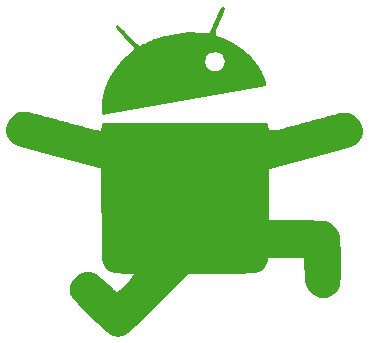
\includegraphics[width=\linewidth]{img/running_bugdroid.png}
      \vfill
    \end{column}
  \end{columns}
\end{frame}
\begin{frame}
  \slidetitle[Debugger]
  \note{\onslide+<1->{\ExecuteMetaData[006-anadyn_notes.tex]{Debugger}}}
  \begin{columns}
    \begin{column}{0.7\linewidth}
      \begin{block}{Principe}<2->
        \begin{enumerate}
        \item<3-> Décompilation de l'application
        \item<4-> Import du projet dans Android Studio
        \item<5-> Mise en place des points d'arrêts
        \item<6-> Lancement du mode debug
        \item<7-> Analyse de l'état de l'application aux points d'arrêts 
        \end{enumerate}
        \begin{itemize}
        \item<8-> Il est par la suite possible de recompiler l'application avec les modifications apportés au smali
        \end{itemize}
      \end{block}
    \end{column}
    \begin{column}{0.25\linewidth}     
      \centering
     \begin{overlayarea}{0.6\linewidth}{\linewidth}
      \only<1-2>{
\includegraphics[width=\linewidth]{0_bugdroid-0.png}}
      \only<3-3|handout:0>{
\includegraphics[width=\linewidth]{img/0_bugdroid-1.png}}
      \only<4-4|handout:0>{
\includegraphics[width=\linewidth]{img/0_bugdroid-2.png}}
      \only<5-5|handout:0>{
\includegraphics[width=\linewidth]{img/0_bugdroid-3.png}}
      \only<6-6|handout:0>{\includegraphics[width=\linewidth]{img/0_bugdroid-4.png}}
      \only<7-7|handout:0>{\includegraphics[width=\linewidth]{img/0_bugdroid-5.png}}
      \only<8-8|handout:0>{\includegraphics[width=\linewidth]{img/0_bugdroid-6.png}}
     \end{overlayarea}
    \end{column}
  \end{columns}

\end{frame}
\end{document}


\framepink
\documentclass[aspectratio=1610]{beamer}%, handout
\usepackage{graphics}
\usepackage{pifont}
\usepackage{ulem}
\usepackage{xcolor}
\usepackage{modifycolor}
\usepackage{lipsum}
\usepackage{fontspec}
\usepackage{caption}
\renewcommand{\figurename}{FIGURE}
\captionsetup[figure]{labelfont={color=leftFootlineColor, scriptsize}, textfont={color=normalBlockColor, scriptsize}}
\usepackage{tabularx}
\newcolumntype{Y}{>{\centering\arraybackslash}X}
\usepackage{tikz}
\usepackage{standalone}
\usepackage{svg}
\usepackage{multicol}
\usepackage{catchfilebetweentags}
\usepackage{xifthen}
\usetikzlibrary{arrows}
\usetikzlibrary{backgrounds}
\setmonofont[
  Contextuals={Alternate}
]{FuraCode Nerd Font}
\setsansfont{Roboto Medium}
\usepackage{pgfpages}


\usepackage[cache=false,outputdir=build]{minted}
\definecolor{bg_code}{HTML}{282828}
\usemintedstyle{darcula}
\setminted{
      fontsize=\scriptsize, 
      linenos,
      numbersep=0pt,
      gobble=5,
      framesep=3mm} 
      \renewcommand{\theFancyVerbLine}{\texttt{{{\arabic{FancyVerbLine}}}}}
\usepackage{adjustbox}
\usepackage{environ}%
\usepackage{tikz}
\usetikzlibrary{patterns}
\usepackage[french]{babel}
\usepackage{beamerthemesideblue}


\setbeamerfont{note page}{size=\footnotesize}
\setbeamertemplate{note page}[custom]
\setbeamercolor{note page}{bg=backgroundColor, fg=white}

\newcommand{\insertlicense}{\includegraphics[height=1cm]{img/by-sa.png}}
\title[]{La rétroingénierie appliquée à Android}
\subtitle{La traque aux traqueurs}
\author{Maxime Catrice}
\date{\today}
\titlegraphic{\includegraphics[height=0.95cm]{logo.png}\bigbreak\insertlicense}

\setbeamertemplate{title page}[default][colsep=-4bp,rounded=true,shadow=false]
\setbeamercolor{background canvas}{bg=backgroundColor}
\setbeamertemplate{blocks}[rounded][shadow=false]
\beamertemplatenavigationsymbolsempty
\newcounter{acolumn}%  Number of current column
\newlength{\acolumnmaxheight}%   Maximum column height
%%%%%%%%%%%%%%%%%%%%%%%%%


\makeatletter

% `column` replacement to measure height
\newenvironment{@acolumn}[1]{%
    \stepcounter{acolumn}%
    \begin{lrbox}{\@tempboxa}%
    \begin{minipage}{#1}%
}{%
    \end{minipage}
    \end{lrbox}
    \@tempdimc=\dimexpr\ht\@tempboxa+\dp\@tempboxa\relax
    % Save height of this column:
    \expandafter\xdef\csname acolumn@height@\roman{acolumn}\endcsname{\the\@tempdimc}%
    % Save maximum height
    \ifdim\@tempdimc>\acolumnmaxheight
        \global\acolumnmaxheight=\@tempdimc
    \fi
}

% `column` wrapper which sets the height beforehand
\newenvironment{@@acolumn}[1]{%
    \stepcounter{acolumn}%
    % The \autoheight macro contains a \vspace macro with the maximum height minus the natural column height
    \edef\autoheight{\noexpand\vspace*{\dimexpr\acolumnmaxheight-\csname acolumn@height@\roman{acolumn}\endcsname\relax}}%
    % Call original `column`:
    \orig@column{#1}%
}{%
    \endorig@column
}

% Save orignal `column` environment away
\let\orig@column\column
\let\endorig@column\endcolumn

% `columns` variant with automatic height adjustment
\NewEnviron{acolumns}[1][]{%
    % Init vars:
    \setcounter{acolumn}{0}%
    \setlength{\acolumnmaxheight}{0pt}%
    \def\autoheight{\vspace*{0pt}}%
    % Set `column` environment to special measuring environment
    \let\column\@acolumn
    \let\endcolumn\end@acolumn
    \BODY% measure heights
    % Reset counter for second processing round
    \setcounter{acolumn}{0}%
    % Set `column` environment to wrapper
    \let\column\@@acolumn
    \let\endcolumn\end@@acolumn
    % Finally process columns now for real
    \begin{columns}[#1]%
        \BODY
    \end{columns}%
}
\makeatother
%%%%%%%%%%%%%%%%%%%%%%%%%

\NewEnviron{frameNoSB}{
\makeatletter
\setbeamertemplate{sidebar canvas left}{}
\setbeamertemplate{sidebar left}{}
\makeatother
\begin{frame}
    \BODY
%\tableofcontents
\end{frame}
}

\NewEnviron{frameTitle}{
\setbeamertemplate{frametitle}[default][center]
\makeatletter
\setbeamertemplate{headline}{\color{backgroundColor}45\newline 45\newline 45\newline 45\newline 45\newline 45\newline 45\newline 45\newline 45\newline 45}
\setbeamertemplate{sidebar canvas left}{}
\setbeamertemplate{sidebar left}{}



\makeatother
\begin{frame}
\begin{minipage}[c]{\linewidth-\beamerleftmargin+\beamerrightmargin}
\BODY
\end{minipage}
\end{frame}
}

\setbeamerfont{title}{series=\bfseries,parent=structure}
\setbeamerfont{subtitle}{size=\Large,series=,parent=structure}

\makeatletter
\newlength\beamerleftmargin
\setlength\beamerleftmargin{\Gm@lmargin}

\newlength\beamerrightmargin
\setlength\beamerrightmargin{\Gm@rmargin}
\makeatother

\newcommand{\nologo}{\setbeamertemplate{logo}{}}

\newcommand{\slidetitle}[1][]{
  \frametitle{\insertsection\ifthenelse{\equal{#1}{}}{}{: #1}}
}
\newcommand{\mono}[1]{
\texttt{#1}
}

\setbeameroption{show notes on second screen=top}
\framegreen
\begin{document}
 

\section{Comment s'en prémunir?}
\begin{frame}
  \slidetitle[La sécurité par l'obscurité]
  \note{\ExecuteMetaData[008-evit_notes.tex]{Obfuscation}}
  \begin{columns}
    \begin{column}[t]{0.48\linewidth}
      \centering
      \begin{block}{Obscurcire son code}<2->
        \begin{itemize}
          \item<3-> Obfuscation de code:
          \begin{itemize}
          \item<4-> Ajout d'instructions inutiles
          \item<5-> Ajout d'arguments inutiles sur les méthodes
          \item<6-> Minimication du code
          \item<7-> Génération dynamique de string
          \end{itemize}
          \item<8-> Chiffrement du programme
          \item<9-> Exécution de code distant
          \end{itemize}
      \end{block}
    \end{column}
    \begin{column}[t]{0.48\linewidth}
      \centering
        \begin{figure}
          \includegraphics[width=\linewidth]{img/obscurity.png}
          \caption{XKCD 257}
        \end{figure}
    \end{column}
  \end{columns}
  \end{frame}
  \begin{frame}
    \slidetitle[L'absurdité de l'obscurité]
    \note{\ExecuteMetaData[008-evit_notes.tex]{Kerckhoffs}}
    \note{\onslide<4->{\ExecuteMetaData[008-evit_notes.tex]{Limites}}}
    \begin{columns}
      \begin{column}{0.48\linewidth}
        \begin{block}{Principe de Kerckhoffs}<2->
          \centering
          \onslide<3->{
          ``Un système est considéré comme étant sécurisé de par sa conception et non parce que sa
          conception est inconnue de l'adversaire''
          }
        \end{block}
        \begin{block}{Les limites de l'obfuscation}<4->
          \begin{itemize}
          \item<5-> Débogage difficile
          \item<6-> Protection temporaire
          \item<7-> Potentiel perte de performances
          \item<8-> Qualité du code en baisse
          \item<9-> Appel à des librairies externes non obfuscables
          \end{itemize}
        \end{block}
      \end{column}
      \begin{column}{0.48\linewidth}
        \includegraphics[width=\linewidth]{img/obscurity.jpg}
      \end{column}
    \end{columns}
    \end{frame}
\end{document}

\frameblue
\documentclass[aspectratio=1610]{beamer}%, handout
\usepackage{graphics}
\usepackage{pifont}
\usepackage{ulem}
\usepackage{xcolor}
\usepackage{modifycolor}
\usepackage{lipsum}
\usepackage{fontspec}
\usepackage{caption}
\renewcommand{\figurename}{FIGURE}
\captionsetup[figure]{labelfont={color=leftFootlineColor, scriptsize}, textfont={color=normalBlockColor, scriptsize}}
\usepackage{tabularx}
\newcolumntype{Y}{>{\centering\arraybackslash}X}
\usepackage{tikz}
\usepackage{standalone}
\usepackage{svg}
\usepackage{multicol}
\usepackage{catchfilebetweentags}
\usepackage{xifthen}
\usetikzlibrary{arrows}
\usetikzlibrary{backgrounds}
\setmonofont[
  Contextuals={Alternate}
]{FuraCode Nerd Font}
\setsansfont{Roboto Medium}
\usepackage{pgfpages}


\usepackage[cache=false,outputdir=build]{minted}
\definecolor{bg_code}{HTML}{282828}
\usemintedstyle{darcula}
\setminted{
      fontsize=\scriptsize, 
      linenos,
      numbersep=0pt,
      gobble=5,
      framesep=3mm} 
      \renewcommand{\theFancyVerbLine}{\texttt{{{\arabic{FancyVerbLine}}}}}
\usepackage{adjustbox}
\usepackage{environ}%
\usepackage{tikz}
\usetikzlibrary{patterns}
\usepackage[french]{babel}
\usepackage{beamerthemesideblue}


\setbeamerfont{note page}{size=\footnotesize}
\setbeamertemplate{note page}[custom]
\setbeamercolor{note page}{bg=backgroundColor, fg=white}

\newcommand{\insertlicense}{\includegraphics[height=1cm]{img/by-sa.png}}
\title[]{La rétroingénierie appliquée à Android}
\subtitle{La traque aux traqueurs}
\author{Maxime Catrice}
\date{\today}
\titlegraphic{\includegraphics[height=0.95cm]{logo.png}\bigbreak\insertlicense}

\setbeamertemplate{title page}[default][colsep=-4bp,rounded=true,shadow=false]
\setbeamercolor{background canvas}{bg=backgroundColor}
\setbeamertemplate{blocks}[rounded][shadow=false]
\beamertemplatenavigationsymbolsempty
\newcounter{acolumn}%  Number of current column
\newlength{\acolumnmaxheight}%   Maximum column height
%%%%%%%%%%%%%%%%%%%%%%%%%


\makeatletter

% `column` replacement to measure height
\newenvironment{@acolumn}[1]{%
    \stepcounter{acolumn}%
    \begin{lrbox}{\@tempboxa}%
    \begin{minipage}{#1}%
}{%
    \end{minipage}
    \end{lrbox}
    \@tempdimc=\dimexpr\ht\@tempboxa+\dp\@tempboxa\relax
    % Save height of this column:
    \expandafter\xdef\csname acolumn@height@\roman{acolumn}\endcsname{\the\@tempdimc}%
    % Save maximum height
    \ifdim\@tempdimc>\acolumnmaxheight
        \global\acolumnmaxheight=\@tempdimc
    \fi
}

% `column` wrapper which sets the height beforehand
\newenvironment{@@acolumn}[1]{%
    \stepcounter{acolumn}%
    % The \autoheight macro contains a \vspace macro with the maximum height minus the natural column height
    \edef\autoheight{\noexpand\vspace*{\dimexpr\acolumnmaxheight-\csname acolumn@height@\roman{acolumn}\endcsname\relax}}%
    % Call original `column`:
    \orig@column{#1}%
}{%
    \endorig@column
}

% Save orignal `column` environment away
\let\orig@column\column
\let\endorig@column\endcolumn

% `columns` variant with automatic height adjustment
\NewEnviron{acolumns}[1][]{%
    % Init vars:
    \setcounter{acolumn}{0}%
    \setlength{\acolumnmaxheight}{0pt}%
    \def\autoheight{\vspace*{0pt}}%
    % Set `column` environment to special measuring environment
    \let\column\@acolumn
    \let\endcolumn\end@acolumn
    \BODY% measure heights
    % Reset counter for second processing round
    \setcounter{acolumn}{0}%
    % Set `column` environment to wrapper
    \let\column\@@acolumn
    \let\endcolumn\end@@acolumn
    % Finally process columns now for real
    \begin{columns}[#1]%
        \BODY
    \end{columns}%
}
\makeatother
%%%%%%%%%%%%%%%%%%%%%%%%%

\NewEnviron{frameNoSB}{
\makeatletter
\setbeamertemplate{sidebar canvas left}{}
\setbeamertemplate{sidebar left}{}
\makeatother
\begin{frame}
    \BODY
%\tableofcontents
\end{frame}
}

\NewEnviron{frameTitle}{
\setbeamertemplate{frametitle}[default][center]
\makeatletter
\setbeamertemplate{headline}{\color{backgroundColor}45\newline 45\newline 45\newline 45\newline 45\newline 45\newline 45\newline 45\newline 45\newline 45}
\setbeamertemplate{sidebar canvas left}{}
\setbeamertemplate{sidebar left}{}



\makeatother
\begin{frame}
\begin{minipage}[c]{\linewidth-\beamerleftmargin+\beamerrightmargin}
\BODY
\end{minipage}
\end{frame}
}

\setbeamerfont{title}{series=\bfseries,parent=structure}
\setbeamerfont{subtitle}{size=\Large,series=,parent=structure}

\makeatletter
\newlength\beamerleftmargin
\setlength\beamerleftmargin{\Gm@lmargin}

\newlength\beamerrightmargin
\setlength\beamerrightmargin{\Gm@rmargin}
\makeatother

\newcommand{\nologo}{\setbeamertemplate{logo}{}}

\newcommand{\slidetitle}[1][]{
  \frametitle{\insertsection\ifthenelse{\equal{#1}{}}{}{: #1}}
}
\newcommand{\mono}[1]{
\texttt{#1}
}

\setbeameroption{show notes on second screen=top}
\framered
\begin{document}
\section{Pourquoi?}

\begin{frame}[t]
  \slidetitle[La traque aux utilisateurs]
  \note{\ExecuteMetaData[009-acteurs_notes.tex]{Traqueurs}}
  \onslide<2->{\includegraphics[height=0.05\linewidth]{img/criteo.pdf}}
  \hfill
  \begin{overlayarea}{0.08\linewidth}{0.08\linewidth}
    \only<4-4|handout:0>{\includegraphics[height=\linewidth]{img/teemo_0.png}}
    \only<5->{\includegraphics[height=\linewidth]{img/teemo_1.png}}
  \end{overlayarea}
  \hfill
  \onslide<3->{\includegraphics[height=0.05\linewidth]{img/fidzup.pdf}}
  \vfill
  \onslide<6->{
  \begin{center}
  ``Retrouver n’importe quel Français prendrait 5 secondes à une équipe de 20 personnes''
  \end{center}}
  \vfill
  \onslide<7->{
  \begin{center}
    ``Le Président de la République est encore plus simple à trouver, car «il est fan de l’Équipe et est toujours suivi par une dizaine d’autres smartphones»''
  \end{center}}
  \vfill
\end{frame}

\begin{frame}
  \slidetitle[La traque aux traqueurs]
  \note{\ExecuteMetaData[009-acteurs_notes.tex]{Defenseurs}}
  \vfill
  \vfill
  \begin{columns}
    \begin{column}{0.15\linewidth}
      \centering
      \vfill
      \onslide<3->{
      \includegraphics[width=0.75\linewidth]{img/exodus.pdf}}
    \end{column}
    \begin{column}{0.7\linewidth}
      \centering
      \begin{block}{Comment savoir qui nous traque?}<2->
        \begin{description}[align left]
          \item<3-> [Exodus Pricacy] Association Française 
          \item<4-> [Yale Privacy Lab] Laboratoire de recherches mêlant vie privée, sécurité et anonimat
          \item<5-> [Kimetrak]Extension Chrome/Firefox pour détecter les traqueurs
        \end{description}
      \end{block}
    \end{column}
    \begin{column}{0.15\linewidth}
      \centering
      \vfill
      \onslide<4->{
    \includegraphics[width=0.75\linewidth]{img/yaleprivacylab.pdf}}
    \end{column}
  \end{columns}
  \vfill
  \onslide<5->{
    \centering
    \includegraphics[width=0.12\linewidth]{img/kimetrak.png}
    }
\end{frame}
\end{document}

\framegreen
\begin{frame}[plain]
  \begin{minipage}{\linewidth-\beamerleftmargin+\beamerrightmargin}
    \begin{block}{}
      \vspace{0.5cm}
      \begin{center}
        {\LARGE{Merci !}}\\
        \pause
        Souriez, vous êtes tracés !
      \end{center}
      \vspace{0.25cm}
  \end{block}
  \bigbreak
  \pause
  \centering
  \url{https://hazegard.github.io/CLOCK/}
  \end{minipage}
\end{frame}
\end{document}